\chapter{Multi-Cell System Performance Analysis under Correlated Shadow Fading}\label{ch:4}
\par In a multi-cell cellular network, connections between the Base Station (BS) and Mobile Users (MUs) may fail when the channel has low signal-to-interference-plus-noise ratio (SINR?. Shadow fading is large-scale fading which can cause significant received power loss and reduce SINR for a wide area. Correlated shadow fading will result in correlated long outage durations. Increasing BS density to make the network become denser is considered to be an efficient way to increase SINR, reduce outage and provide better Quality of Service (QoS) support for delay sensitive applications in noise-limited regime. This chapter is an extension of Chapter \ref{ch:ExpSingleCell}, which focuses on the study of the performance of a multi-cell communication system under correlated shadow fading. We consider the downlink direction in a multi-cell communication system. To investigate the outage probability given correlated shadow fading and different BS densities, two system layouts, Grid model and Random model, are studied. First, we compare the outage probability with same correlated shadow fading with regard to the two different system layout. Simulation results indicate that grid model performs better than Random model. Secondly, the outage probability with independent shadow fading and with correlated shadow fading for Random model are compared. SINR is calculated by assuming shadow fading follows independent identical distributed (\emph{i.i.d}) Gaussian and jointly distributed Gaussian shadow fading. Thirdly, we focus on Random model which is more realistic and presented the outage duration under two circumstances: independent shadow fading and correlated shadow fading. Simulation results show that outage durations with correlated shadow fading are longer than those with the independent shadow fading. At last, we showed that increasing BS density can mitigate the effect of correlated shadow fading and improve the system performance by reducing outage probability and outage duration. 
\section{Background}
%\par In a cellular communication system, the connection between the BS and a MU may be dropped when the user enters a deeply shadowed area. Fading phenomena can substantially affect the performance of a wireless communication system. In general, fading can be divided into two categories: large-scale fading and small-scale fading. A signal transmitted from source to destination will experience both large-scale and small-scale fading. Small-scale fading is caused by multipath propagation. Large-scale fading, which is also known as shadow fading, is caused by obstacles (trees, buildings, etc.) in the propagation path. In most cases, shadow fading is assumed to be temporally and spatially independent \cite{rappaport1996wireless}.  Researchers have also shown that shadow fading is spatially correlated at different positions on the propagation path \cite{gudmundson1991correlation}, \cite{zhang2008novel}. In \cite{fabbri2009impact} and \cite{patwari2008effects}, the effects of correlated shadowing in connectivity is demonstrated, which indicates that reliable connectivity will be much more difficult to maintain than indicated by independent shadow fading models. The spatial correlation of shadow fading is important when studying the quality of service of a mobile system since it will result in long-lasting outage durations, which will deteriorate the performance of the applications running on the network. The focus of this chapter is to study channel variations and system performance due to correlated shadow fading in a multi-cell communication system and provide a solution to reduce the frequency and duration of dropped connections and improve system performance by increasing BS density.
\par There have been a lot of studies on the outage probability of cellular communication systems \cite{abu1991outage, petrovic2013outage, emamian2014outage}. The author of \cite{vural2015effect} analyzed the outage probability and coverage area under \emph{i.i.d} shadow fading distributions: Log-normal distribution, Weibull distribution and Gamma distribution. In contrast, there is much less work on the outage probability and outage duration given correlated shadow fading. The system performance of multi-cell system given correlated shadow fading is still an open problem. In \cite{lu2015long} and \cite{lu2015shining} we studied the outage probability and outage duration of a single-cell communication system under exponentially correlated shadow fading and distance-angle correlated shadow fading. \cite{lu2015long} we showed that for a single cell model, exponentially correlated shadow fading can be modeled as a Markov Chain Model. Highly correlated shadow fading will result in long-lasting outage durations. In \cite{lu2015shining}, single-cell model given distance-angle correlated shadow fading system is studied. The correlated shadow fading leads to correlated outage and long outage durations in a single cell model. We provided a solution to overcome the correlated shadow fading: relay cooperative communication. Chapter \ref{ch:CoopComm} and Chapter \ref{ch:ExpSingleCell} are limited to single-cell model. In this chapter, we are going to extend the study to correlated shadow fading impact on a multi-cell communication system, and provide a solution to overcome the long-lasting outage duration.
\par For multi-cell system, in \cite{andrews2011tractable}, the author developed a new general model for the multi-cell SINR using stochastic geometry. The cellular network is modeled by placing the BSs at locations as a homogeneous Poisson Point Process. The author concluded that under general fading, increasing the number of BSs does not affect the coverage probability (so is the outage probability) while the MU is connected to the nearest BS. The paper also did comparison between grid model and the random PPP model and concluded that a regular grid model provided the upper bound of the coverage probability while the PPP provided the lower bound. The author also considered the effect on independent log-normal interference and concludes that the increasing log-normal interference increased the coverage probability which seems counter-intuitive. In that paper, the author didn't consider the scenarios with correlated log-normal interference. Nevertheless, only the coverage probability is studied, analysis of outage duration has not been analyzed. 
\par A comparative study of random and grid topology of small cell network deployment was given in \cite{chen2012small}. In this paper, spatial outage probability and spatial average throughput versus the number of access points of the two different network deployment is studied. However this paper considered independent log-normal interference instead of correlated log-normal fading. Approximate outage probability and capacity for $\kappa-\mu$ shadow fading is studied in \cite{kumar2015approximate}. $\kappa-\mu$ shadow fading includes one-side Gaussian, the Rayleigh, the Nakagami-m, the Rician. As we mentioned before, the imperial measurements didn't exhibit such complicated features of shadow fading. Therefore when investigating system performance under correlated shadow fading, those complex features are not of main focus.
\par The key contributions of this chapter are summarized as below:
\begin{itemize}
\item Correlated outage fields are given to analyze the relationship between correlated shadow fading and correlated outage events. 
\item Investigate outage probability of both Grid model and Random model given correlated shadow fading.
\item Show how increasing BS densities help mitigate correlated shadow fading for Random model in terms of outage probability (coverage probability) and outage durations.
\item Analyze the relation between the tunable parameter of the correlated shadow fading model and the outage probabilities.
\item Compare the system performance of different MU-BS connection strategies: MU connecting to the nearest BS and MU connecting to the BS providing strongest signal.
\end{itemize}
The chapter is organized as follows: Section \ref{ch:CorrShadowField} presents the correlated shadow fading model that is used in this paper and the resultant correlated outage field. Section \ref{SystemModel} presents the system model with two different BS deployment schemas and investigates the outage probability given different BS layout models. Section \ref{OutageProb} gives theoretical analysis of outage probability given correlated shadow fading. Section \ref{SimuProb} presents the simulation setup and analyzes the simulation results of different BS densities. Section \ref{ch4:Conclusion} summarizes the chapter and proposes future work directions.
\section{Correlated Shadow Fading}
\label{CorrShadowField}
As stated in the Chapter \ref{ch:CoopComm}, empirical measurement shows that there exist different patterns of correlations between the shadowing. The independent log-normal shadow fading model, while very useful for static MS performance analysis, cannot reflect the correlation of shadow fading between different locations. In this section, we will give a brief introduction of shadow fading models, including the model used in this chapter.
In Chapter \ref{ch:CoopComm}, a distance-angle correlation model is used and in Chapter \ref{ch:ExpSingleCell} an exponential correlation model is used. The correlation matrix of distance-angle model is given below:
\begin{equation}
\mathbf{K}_{N\times N} = [ \sigma_{s}(\vec{r_{i}})\sigma_{s}(\vec{r_{j}})h(\vec{r_{i}}\vec{r_{j}})],
\label{correlationmatrix}
\end{equation}
where $N$ paths interfere with path $\vec{r_{i}}$ and $\mathbf{E}\{S_{i}^{2}|\vec{r_{i}}\}=\sigma_{s}^{2}(\vec{r_{i}})$. This model assumes that in the correlation matrix, $h$ is separable with respect to the angle of arrival
\begin{equation}
\theta = |\angle\vec{r_{i}}-\angle\vec{r_{j}}|\in [0^{\circ},180^{\circ}],
\end{equation}
and the arrival distance ratio
\begin{equation}
R=|10\log_{10}r_{i}/r_{j}|=\frac{10}{\ln 10}|\ln r_{i}-\ln r_{j}|,
\end{equation}
\begin{equation}
h(\vec{r_{i}},\vec{r_{j}})=max\{1-\theta/\theta_{0},0\}\cdot max\{1-R/R_{0},0\}.
\label{eq:1}
\end{equation}
The correlation coefficients is a piece-wise linear function (\ref{eq:1}) of the angle of arrival and the arrival distance ratio. This correlation model is perfect for single-cell model when there is only one BS at the center of the cell. However, considering multi-cell system, there are quite a number of BSs at different places, both auto-correlation and cross-correlation need to be taken care of. It is not possible to choose a single BS as the center of the shadowing field. To incorporate both auto-correlation and cross-correlation, the simulation complexity will increase in dramatic order. Due to this feature, the distance-angle model is not suitable for analyzing mulit-cell system performance. In this chapter, we use the exponentially correlated shadow fading model \cite{szyszkowicz2011interference} the same as in Chapter \ref{ch:ExpSingleCell}. In \cite{szyszkowicz2011interference}, the author states that correlation in shadowing is indispensable for the analysis of interference of large networks. An exponentially correlated shadowing field $S$ with shadow fading factor $s_{i}$ for each position $p_{i}$ has a correlation matrix as below:
\begin{equation}
\mathbf{K}_{N\times N} = [ \sigma_{s}(p_{i})\sigma_{s}(p_{j})\rho(i,j)],
\label{correlationmatrix}
\end{equation}
where $N$ is the length of the shadowing field. Suppose $A$ and $B$ are two neighbouring points, the shadow fading (in dB) is $N(0,\sigma^2)$ where $\sigma$ is the standard deviation. The spatial correlation between $s_{A}$ and $s_{B}$ will be given by 
\begin{equation}
\rho_{A,B} = \frac{E[s_{A}s_{B}]}{\sigma^2} =e^{-\frac{d_{A,B}}{d_{0}}}
\end{equation}
\begin{figure}
\centering
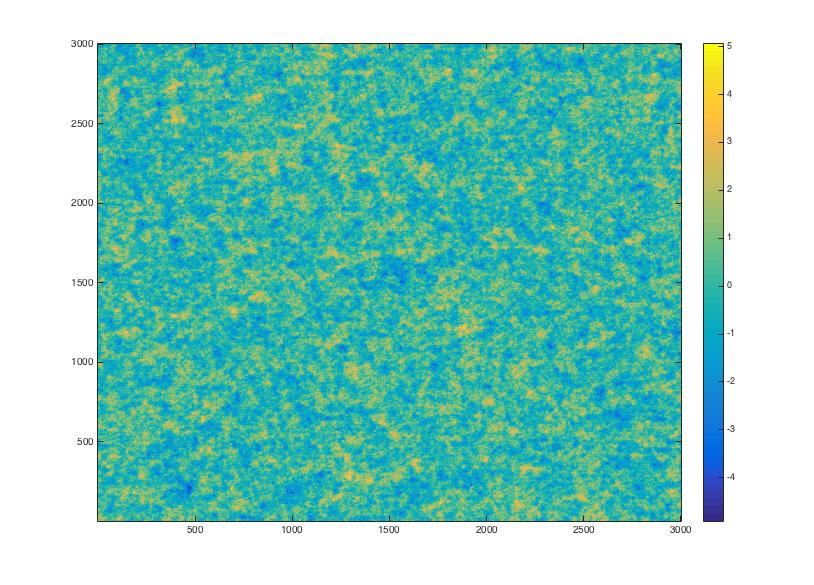
\includegraphics[width = 10cm]{ShadowFieldDeCorr20.jpg}
\caption{Exponentially correlated shadowing field with $d_{0} = 20m$ (the color of the area refers to the normalized standard deviation which is $S_{i}/\sigma_{s}(i)$)}

\label{ch4:shadowingfield}
\end{figure}

Following the shadowing field generation algorithm, we generate shadowing fields with different values of de-correlation distances. A sample shadowing field is shown in Figure \ref{ch4:shadowingfield}.

\par Given a correlated shadowing field, the outage events at different locations are also correlated. Without considering other small-scale fading, the channel gain at different locations has a spatial correlation. Given a proper threshold $\gamma$, an outage area is defined as channel gain less than $\gamma$. Based on the aforementioned correlated shadow fading model and Random system model, a correlated outage filed can be generated as in Figure \ref{outagefie}. On the left, an outage field with independent log-normal shadow fading is shown while the correlated outage field with correlated shadow fading is given on the right. The black color indicates outage areas. Outage area with i.i.d. shadow fading are nonconsecutive dots while with correlated fading are connected areas. This demonstrates correlated outage areas come with correlated shadow fading.

\begin{figure*}
\centering
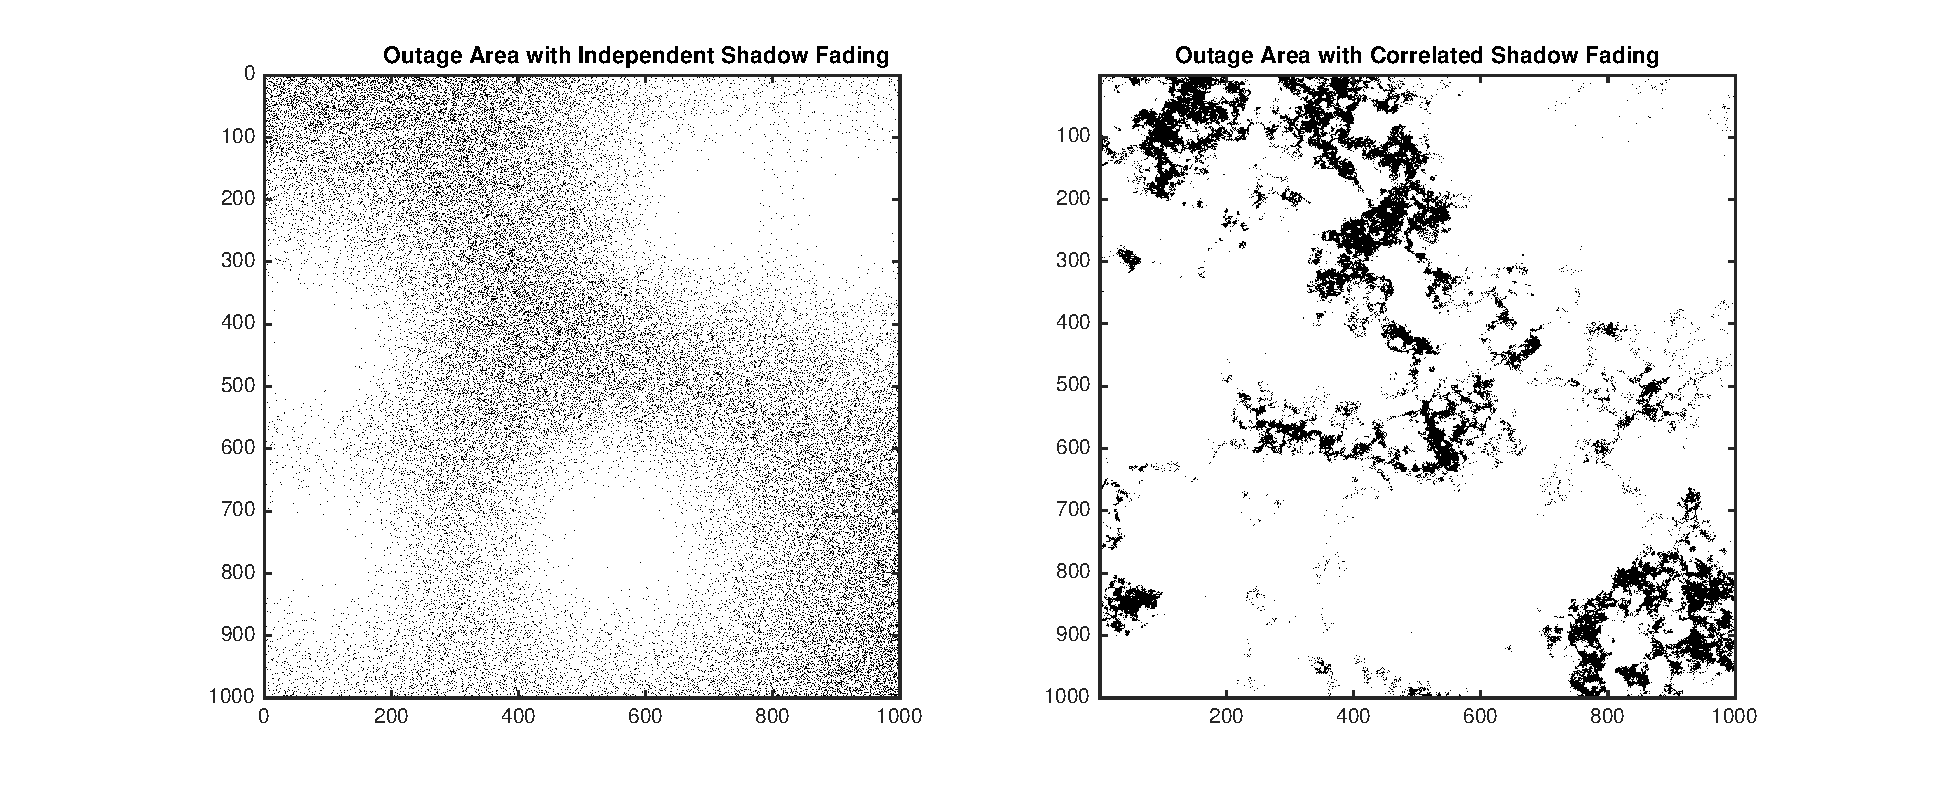
\includegraphics[width=14cm]{outageArea.eps}
\caption{Correlated Outage Fields with $\gamma$ (Dark areas are outage areas while white areas are non-outage areas)}
\label{outagefie}
\end{figure*}


\section{System Model}
\label{SystemModel}
In this paper, we considered two system models with two different BS deployment scheme: Grid model and Random model.
\begin{itemize}
\item Grid Model: $\lambda$ BSs are placed on a regular grid deterministically.
\item Random Model: $\lambda$ BSs are placed randomly in a fixed area.
\end{itemize}
\begin{figure}
\centering
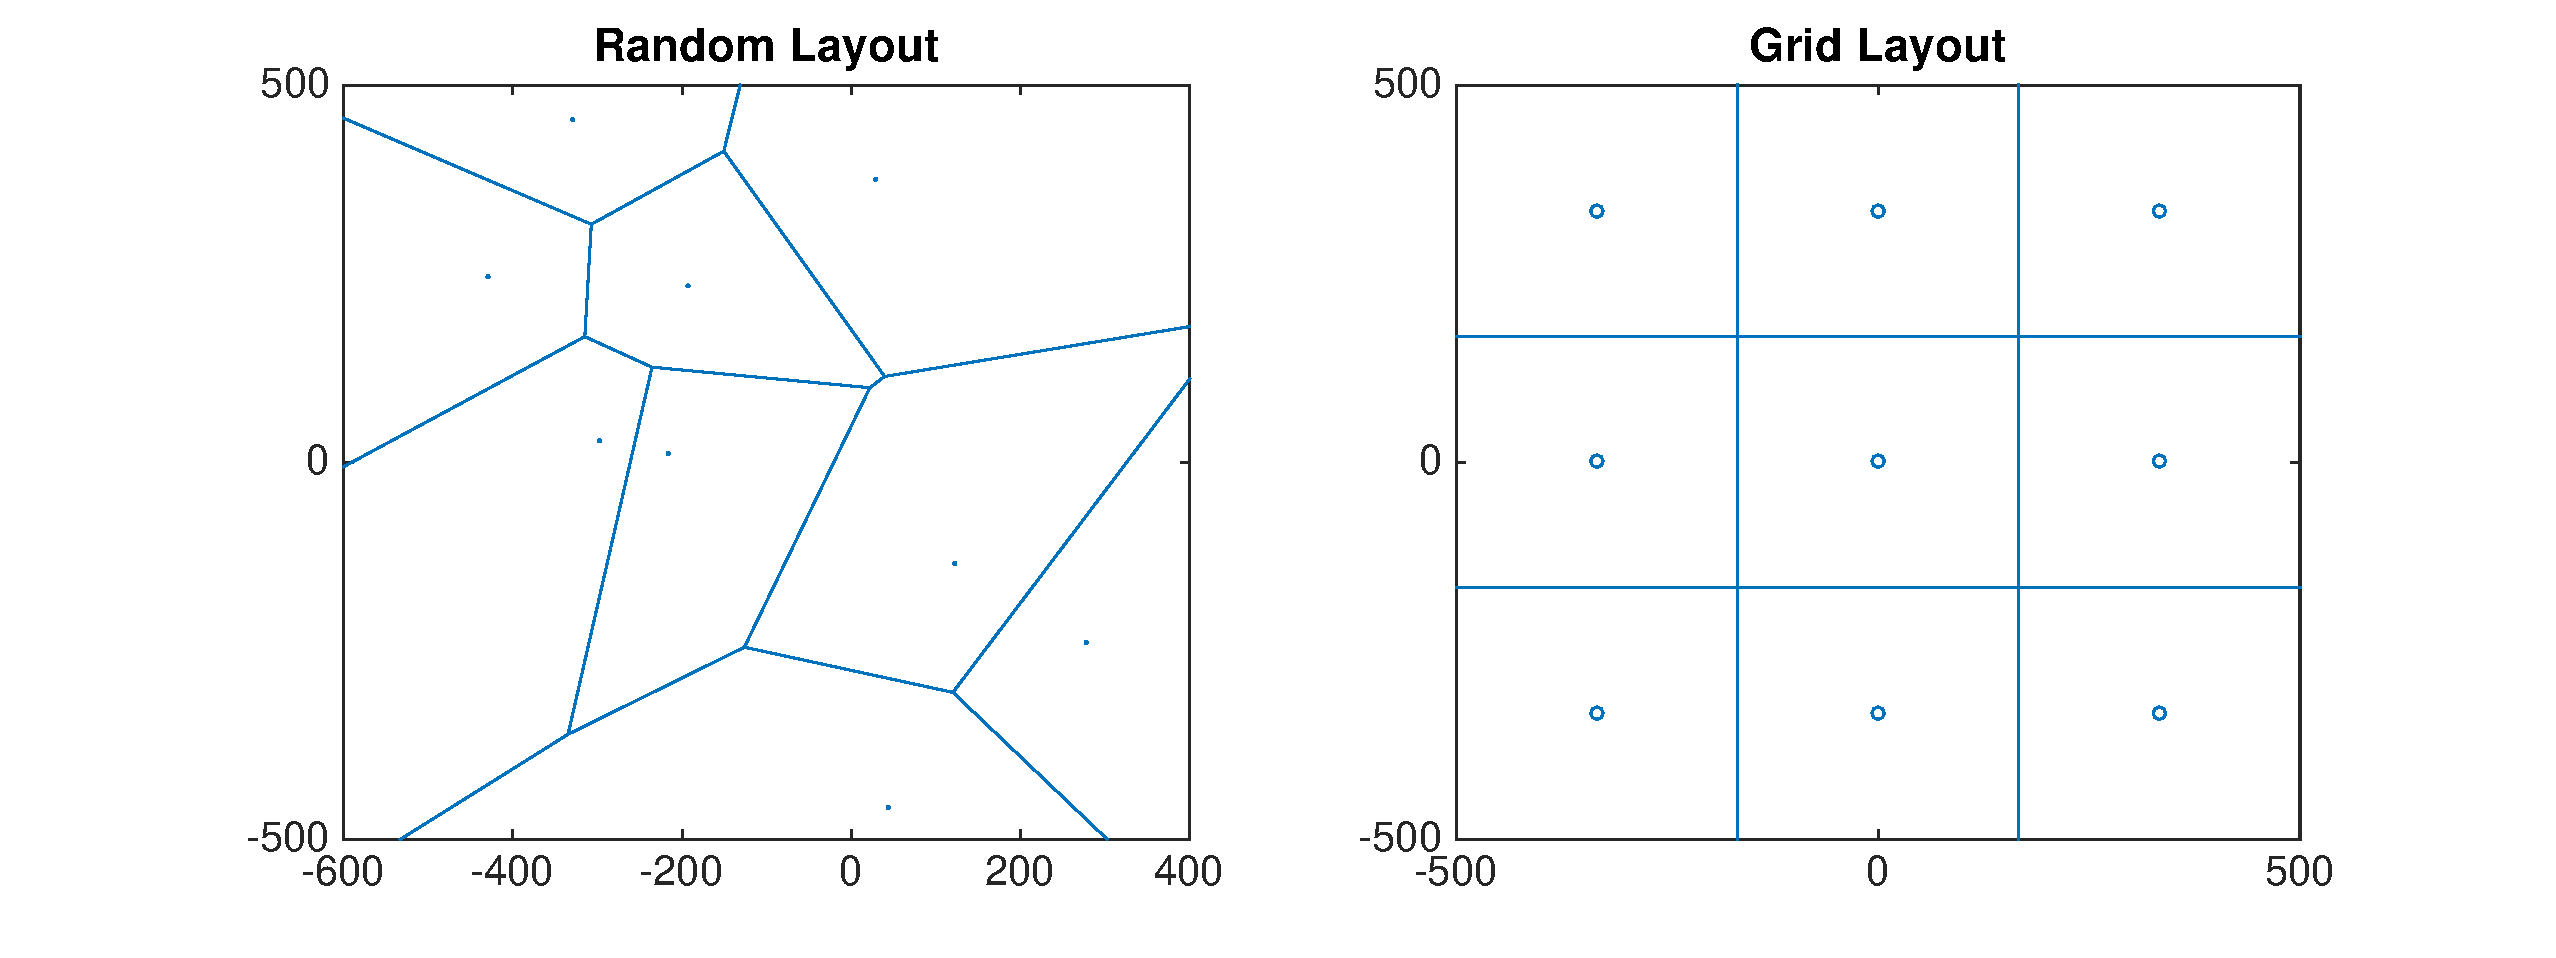
\includegraphics[width=14cm]{systemLayout.eps}
\caption{Random Layout and Grid Layout with $\lambda = 9$.}
\label{RandomLayout}
\end{figure}
% \begin{figure}
% \centering
% \includegraphics[width=8cm]{GridLayout.eps}
% \caption{Grid Base Station Locations}
% \label{GridLayout}
% \end{figure}
Left subfigure of Fig \ref{RandomLayout} is an example of the traditional grid model, where cells are in regular square shape with same size. For the Random model showed in Fig \ref{RandomLayout} right subfigure, cells are not guaranteed to be the same shape and same size. Nearest distances between different cells are in a large variation. 


\section{Outage Probability Analysis}
\label{OutageProb}
\par Let $\varphi = \{1, 2, \dots, N\}$ denotes the set of all Base Stations, then the received signal from Base Station $j$ to the destination user $D$ is given by:
\begin{equation}
y_{i\to D} = G_{i\to D}x_{i}+n_{D}.
\end{equation}
where $x_{i}$ is the signal transmitted by the source Base Station and $y_{i\to D}$ is the signal received by the destination. $n_{D}\sim \mathcal{CN}(0,N_{0})$ is additive white Gaussian noise. $G_{i\to D}$ is the channel gain from source Base Station to destination including path loss and shadow fading. The end-to-end received signal-to-interference-plus-noise ratio $\text{SINR}$ is given as follows:
\begin{equation}
\text{SINR} \triangleq \frac{P_{i}*G_{i\to D}^{2}}{N_{0}+\sum_{j\in \varphi/i}P_{j}*G_{j\to D}^2},
\end{equation}
where $P_{i}$ is the transmitted power of Base Station $i$. The destination successfully receives the signals if no outage event happens, i.e., $\log_{2}(1+\text{SINR})\ge R$, where $R$ is the required data rate. From the definition of SINR, no outage event happens as long as $\text{SINR} > \gamma$, where $\gamma = 2^{R}-1$.

\par For a particular MU, outage happens when its received SINR is less than a threshold to decode the received signal. In our scenario, the probability that the receiver cannot decode signals received from its serving Base Station is defined as:
\begin{equation}
P(out_{i}) = P[\text{SINR}_{i\to D} < \gamma],
\end{equation}
We investigate two connection strategies: 
\begin{itemize}
\item Nearest BS: MU choose to connect to the nearest BS.
\item Strongest BS: MU choose to connect to the BS providing strongest signal.
\end{itemize}
\par In Nearest BS mode, we assume that the user is served by the nearest Base Station, then the outage probability will be 
\begin{equation}
P_{out} = P_{out_{i}},
\end{equation} 
where $i$ is the index of the nearest Base Station. 
\par In Strongest BS mode, under the assumption that an MS always connecting to the Base Station which provides the best received signal, the outage event happens if no Base Station can provide big enough SINR to the receiver. Based on this assumption we have:
\begin{equation}
P_{out} = \max_{i = 1,\cdots,N} P[\text{SINR}_{i\to D}<\gamma].
\end{equation}
The probability density function (pdf) of shadow fading $S$ given $L$ correlated fading branches is
\begin{equation}
\begin{split}
f_{\mathbf{S}}(\mathbf{s}) = &\frac{\lambda^{L}}{\sqrt{2\pi}|\mathbf{K}_{L\times L}|^{1/2}\prod_{i=1}^{L}s_{i}}\\
&\cdot\exp(-\frac{1}{2}(10\log_{10}\mathbf{s}-\boldsymbol{\mu})^{T}\mathbf{K}_{L\times L}^{-1}(10\log_{10}\mathbf{s}-\boldsymbol{\mu})),
\end{split}
\end{equation}
where $\lambda = 10/\ln10$ and $\boldsymbol{\mu}$ is the average shadow fading which is normally $0$. $\mathbf{K}_{L\times L}$ is the correlation matrix which is defined in \eqref{correlationmatrix}. Let $\theta_{i} = \frac{10\log_{10}s_{i}-\mu_{i}}{\sqrt{2}\sigma_{i}}$, and doing a change of variables gives us the pdf of $\mathbf{\Theta}$ as follows:
\begin{equation}
f_{\mathbf{\Theta}}(\boldsymbol{\theta}) = \frac{1}{\pi^(L/2)|\mathbf{\Sigma}|^{1/2}}\exp(-\mathbf{\Theta}^{T}\mathbf{\Sigma}^{-1}\mathbf{\Theta}),
\end{equation}
where $\mathbf{\Sigma}$ is the correlation coefficient matrix which is
\begin{equation}
\left[\begin{array}{cccc}
1 & h_{1,2} & \cdots & h_{1,L}\\
\vdots & \ddots & \ddots & \vdots\\
h_{L,1} & h_{L,2} & \cdots & 1\\
\end{array}\right].
\end{equation}
Since $\text{SINR}_{i\to D}=PL_{i\to D}+S_{i}-N_{0}-\sum_{j\in\varphi/i}(PL_{j\to D} + S_{j})$ in dB, $\text{SINR}_{i\to D}<\gamma$ means
\begin{equation}
S_{i} - \sum_{j\in\varphi/i}S_{j}<\gamma -PL_{i\to D} + \sum_{j\in\varphi/i}PL_{j\to D} + N_{0},
\end{equation}
Then with the assumption that users are served by the nearest Base Station or the best channel Base Station, the outage probability can be written as:
\begin{equation}
\label{outprob}
P_{out} = \underbrace{\int_{-\infty}^{+\infty}\cdots\int_{-\infty}^{+\infty}}_{i =1,\cdots,N} g(PL_{i}S_{i} - \gamma\sum_{j\in\varphi/i}PL_{j}S_{j})f(\mathbf{s})d\mathbf{s}.
\end{equation}
where $\mathbf{s}$ is the correlated shadow fading experienced by all Base Stations, $g(PL_{i}S_{i} - \gamma\sum_{j\in\varphi/i}PL_{j}S_{j})$ is a step function defined in (\ref{stepfunction}).
\begin{figure}[!t]
% ensure that we have normalsize text
\normalsize
% Store the current equation number.
% \setcounter{MYtempeqncnt}{\value{equation}}
% % Set the equation number to one less than the one
% % desired for the first equation here.
% % The value here will have to changed if equations
% % are added or removed prior to the place these
% % equations are referenced in the main text.

\begin{equation}
\label{stepfunction}
g(PL_{i}S_{i} - \gamma\sum_{j\in\varphi/i}PL_{j}S_{j}) = \{\begin{array}{cc}
               1, &  \text{  when }PL_{i}S_{i} - \gamma\sum_{j\in\varphi/i}PL_{j}S_{j} <\frac{\gamma N_{0}}{P}\\
               0, & \text{  when }PL_{i}S_{i} - \gamma\sum_{j\in\varphi/i}PL_{j}S_{j} >\frac{\gamma N_{0}}{P}
             \end{array}.
\end{equation}
% Restore the current equation number.
% \setcounter{equation}{\value{MYtempeqncnt}}
% IEEE uses as a separator
\hrulefill
% The spacer can be tweaked to stop underfull vboxes.
\vspace*{4pt}
\end{figure}

\section{Simulation Results}
\label{SimuProb}
\par In this section, we will present simulation setup and results. First, we run simulations to compare the outage probability of the two different network topology: Grid model and Random model. Secondly, SINR distribution and outage probability of Random model given different BS densities are investigated. Two scenarios are considered: MU connecting to the nearest BS and MU connecting to the BS providing strongest signal. At the end, the outage duration distribution are simulated and discussed given different BS densities. The values of parameters that are used in the simulation are shown in Table \ref{SystemConfig2}. 
\begin{table}
\centering
\caption{\label{SystemConfig2}Simulation Configuration Parameters}

\begin{tabular}{|c|c|}

\hline
Study Area & $1000m\times 1000m$\\
\hline
BS Densities & $3, 10, 50, 100, 200, 300, 500$\\
\hline
Pathloss Exponent & $4$\\
\hline
BS Transmission Power & $P: 40dbm$\\
\hline
SNR Requirement & $-5dB$\\
\hline
De-Correlation Distance & $20m, 200m$\\
\hline
\end{tabular}

\end{table}

\par Figure \ref{cdf1} shows the Cumulative Distribution Function (CDF) of SINR when MU connecting to the nearest BS. The de-correlation distance of the correlated shadow fading is $20m$. The figure suggests that Grid model outperforms the Random model, which is consistent with findings in \cite{andrews2011tractable}. Figure \ref{outage1} shows the outage probability with SINR threshold $-5dB$. The outage probability of Grid Layout (blue) is lower than the Random Layout (yellow). In next section, we will focus on the Random model which is realistic than Grid model.
\begin{figure}
\centering
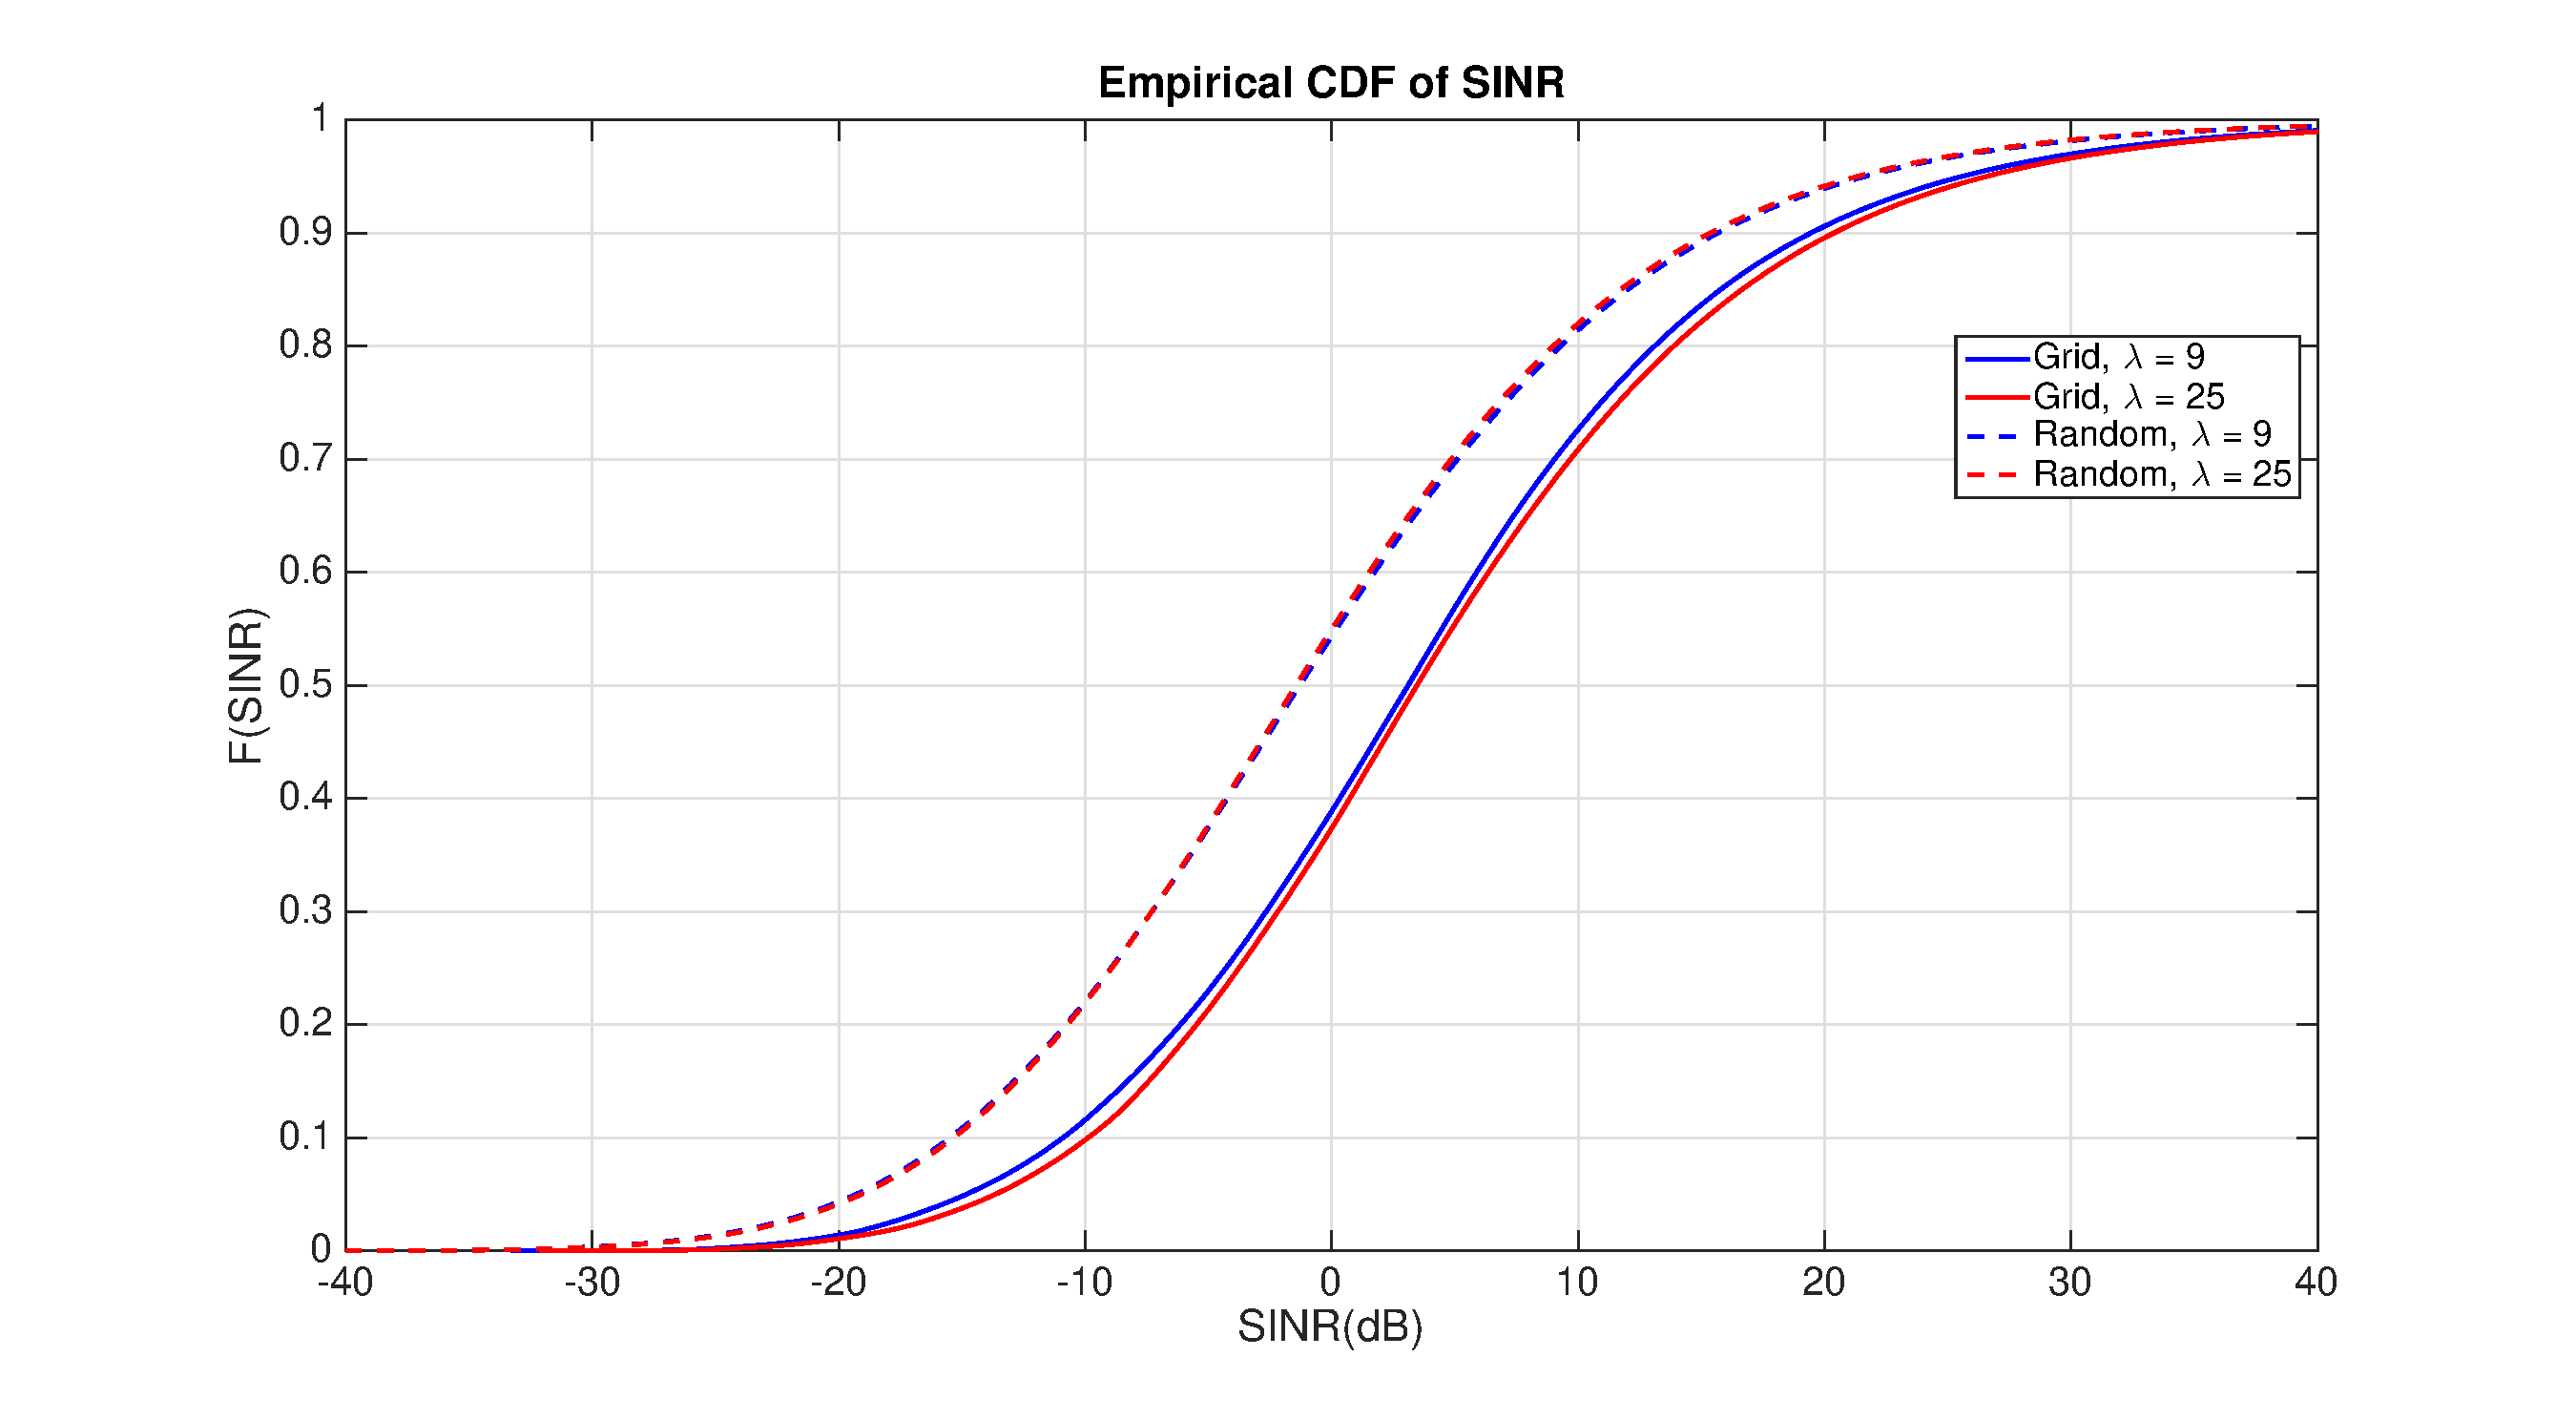
\includegraphics[width=10cm]{GridVSRandom.eps}
\caption{CDF of SINR given Grid Layout and Random Layout (De-Correlation Distance: $20m$)}
\label{cdf1}
\end{figure}
\begin{figure}
\centering
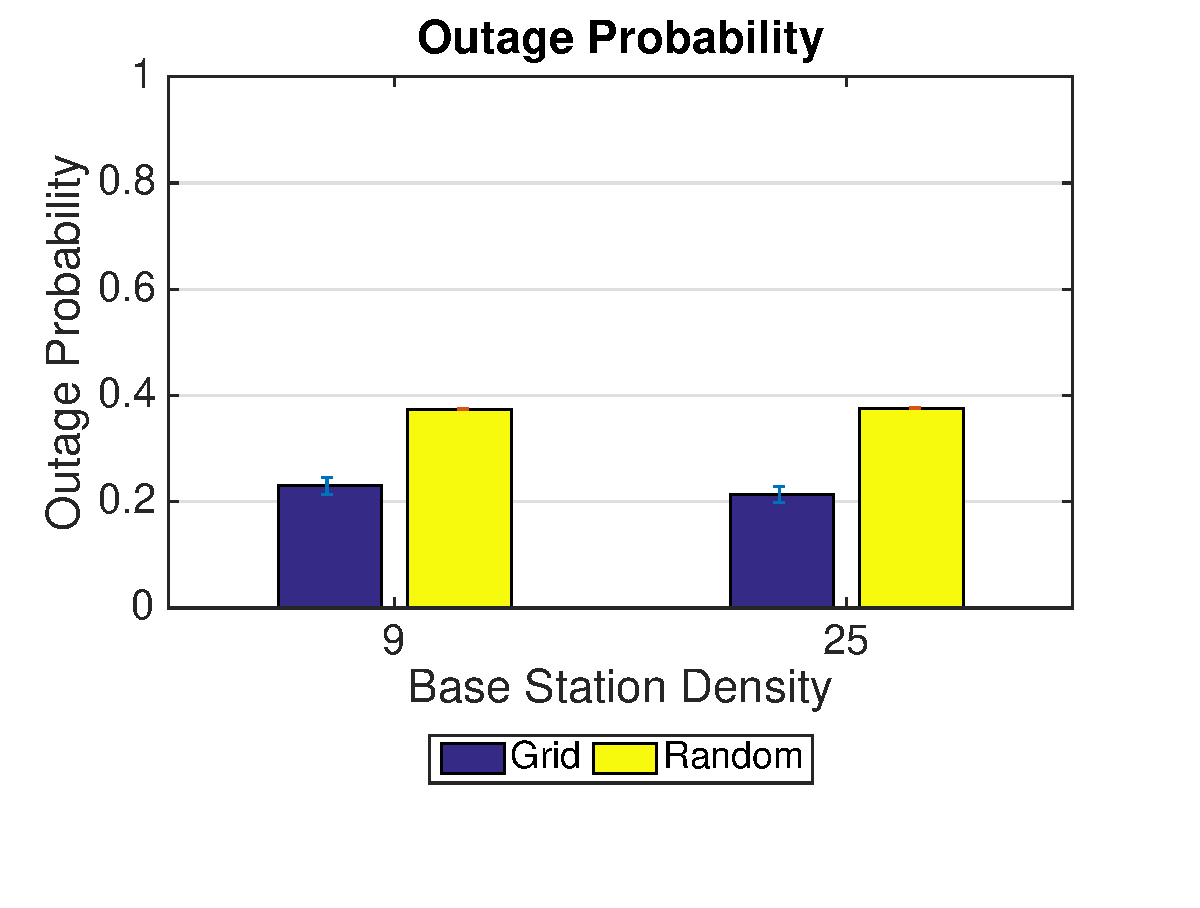
\includegraphics[width=10cm]{OutageProbGridVSRandom.eps}
\caption{Outage Probability given Grid Layout and Random Layout (De-Correlation Distance: $20m$)}
\label{outage1}
\end{figure}


\begin{figure}
\centering
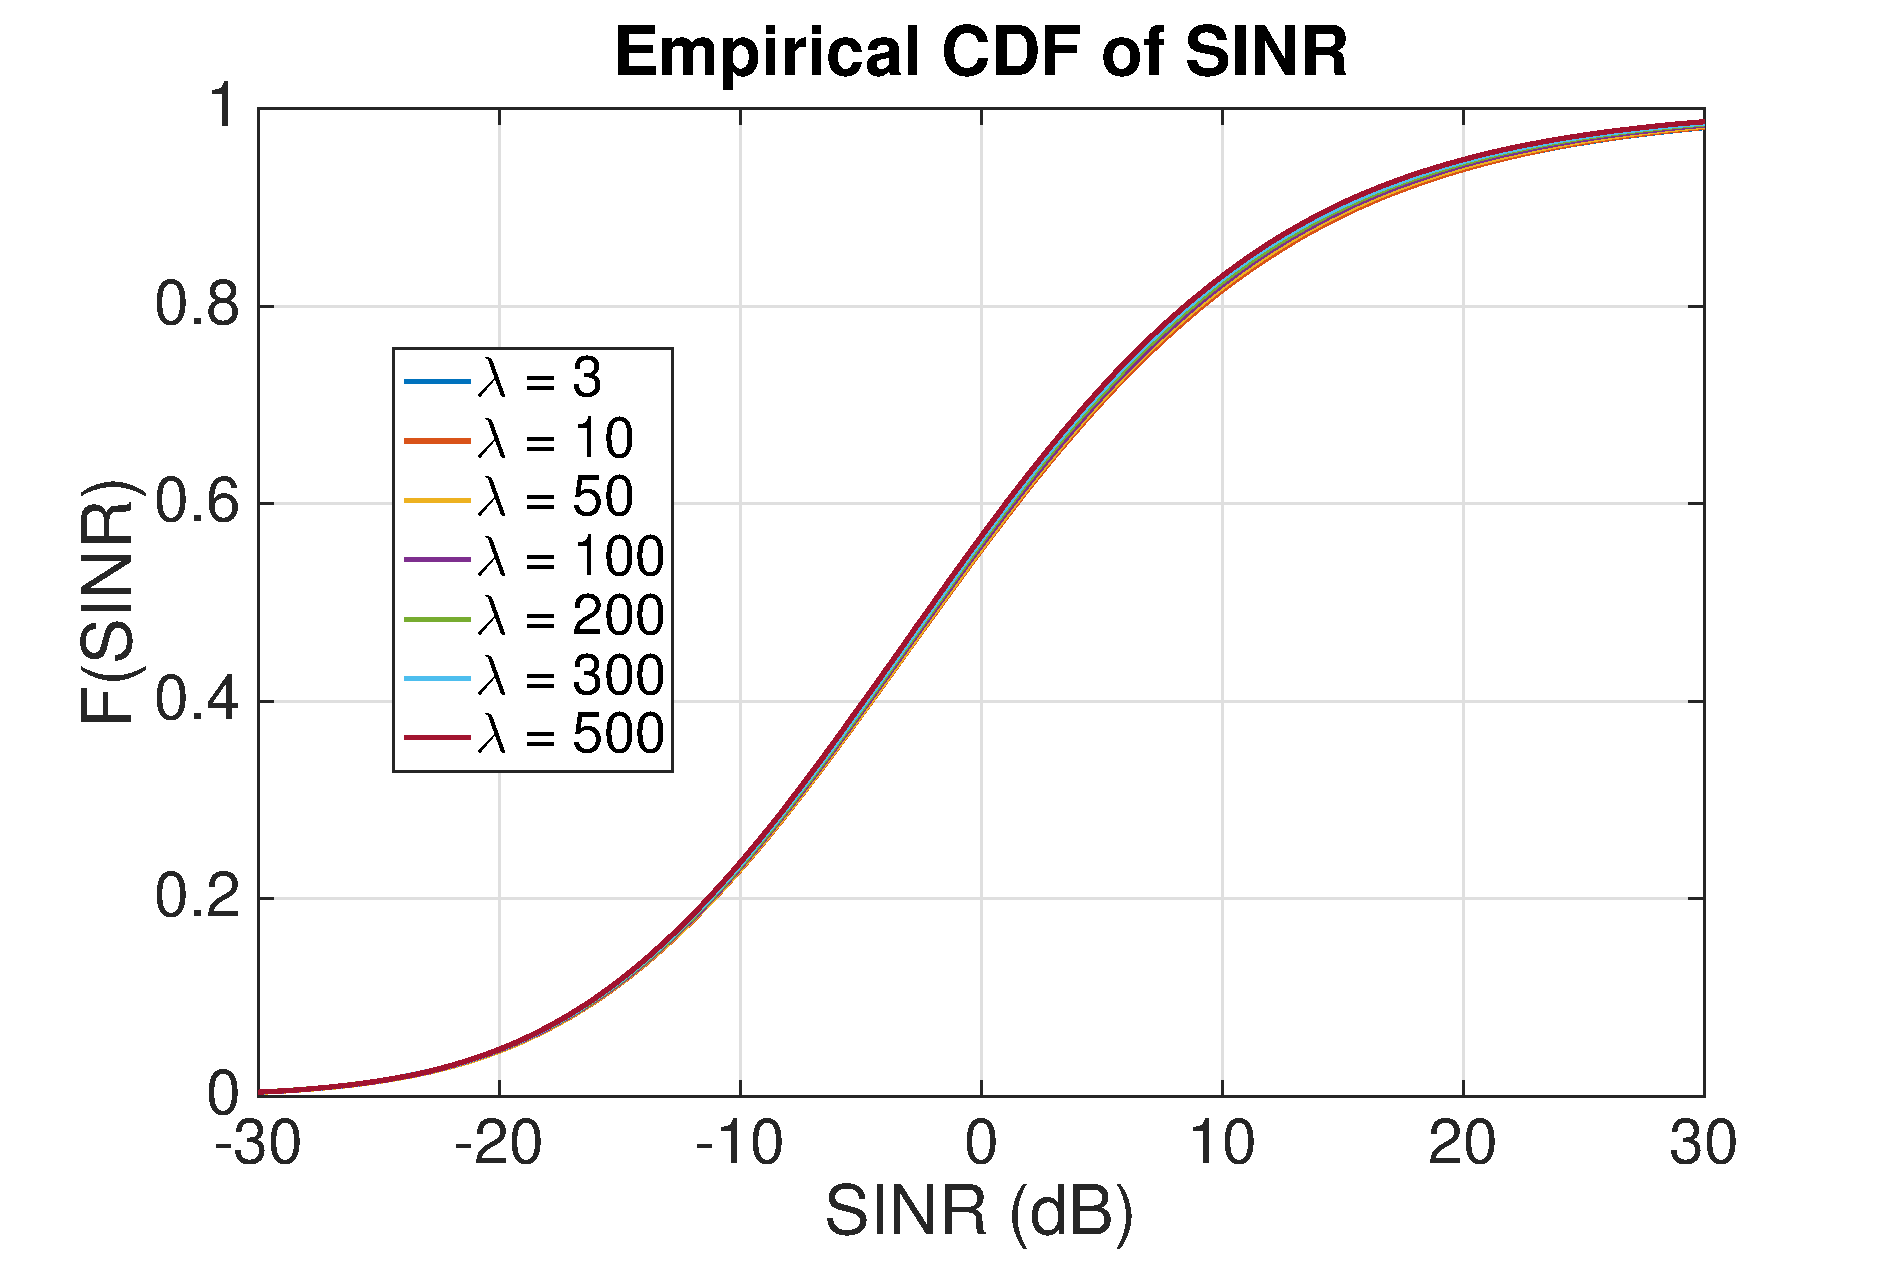
\includegraphics[width=10cm]{NBMax1000OutageProbCDFiid.eps}
\caption{CDF of SINR of MU when connecting to the nearest BS. i.i.d. Shadow Fading}
\label{Mode1}
\end{figure}
\begin{figure}
\centering
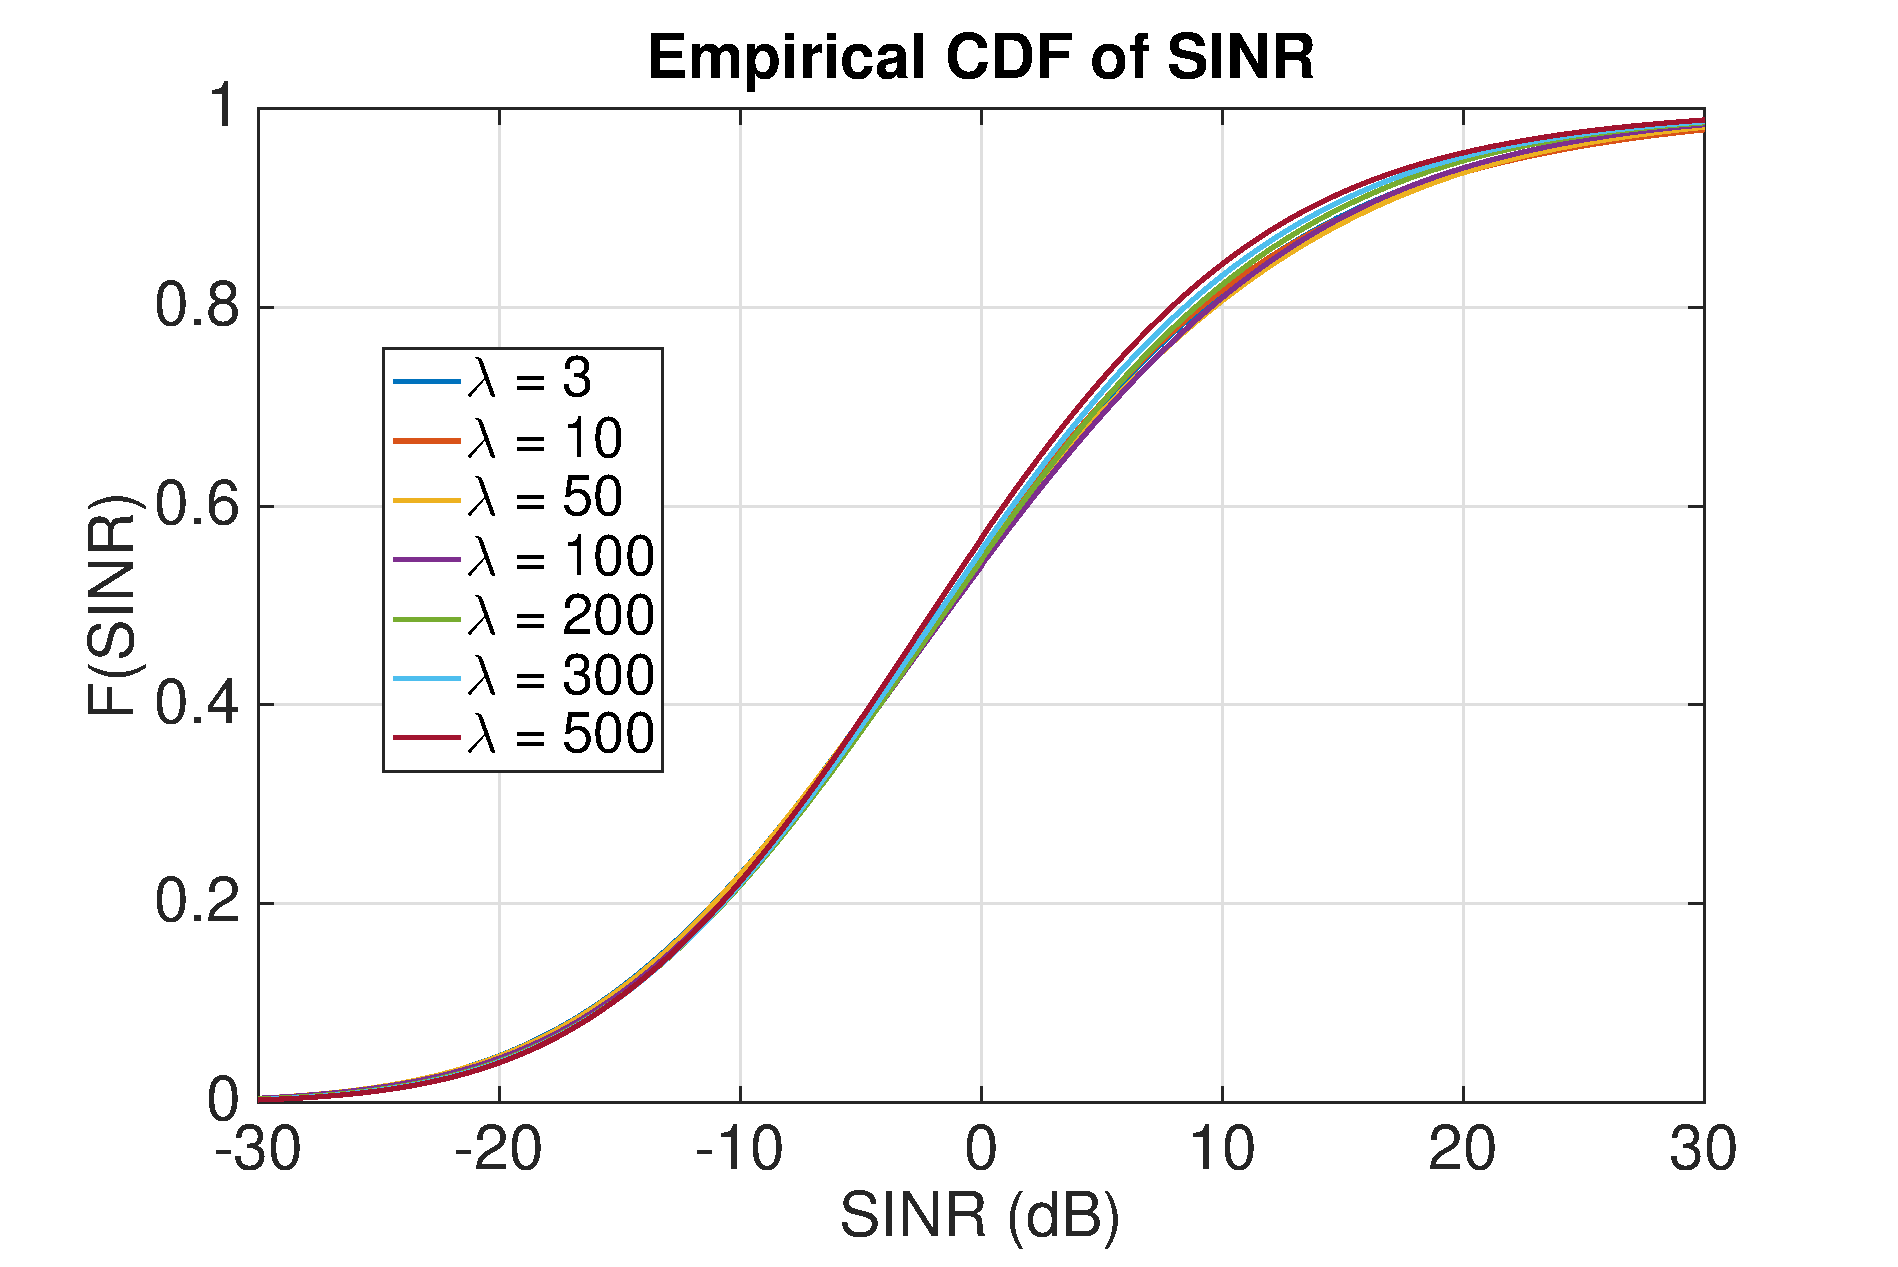
\includegraphics[width=10cm]{NBMax1000OutageProbCDFDeCorr20.eps}
\caption{CDF of SINR of MU when connecting to the nearest BS. De-Correlation Distance: 20m}
\label{Mode2}
\end{figure}
\begin{figure}
\centering
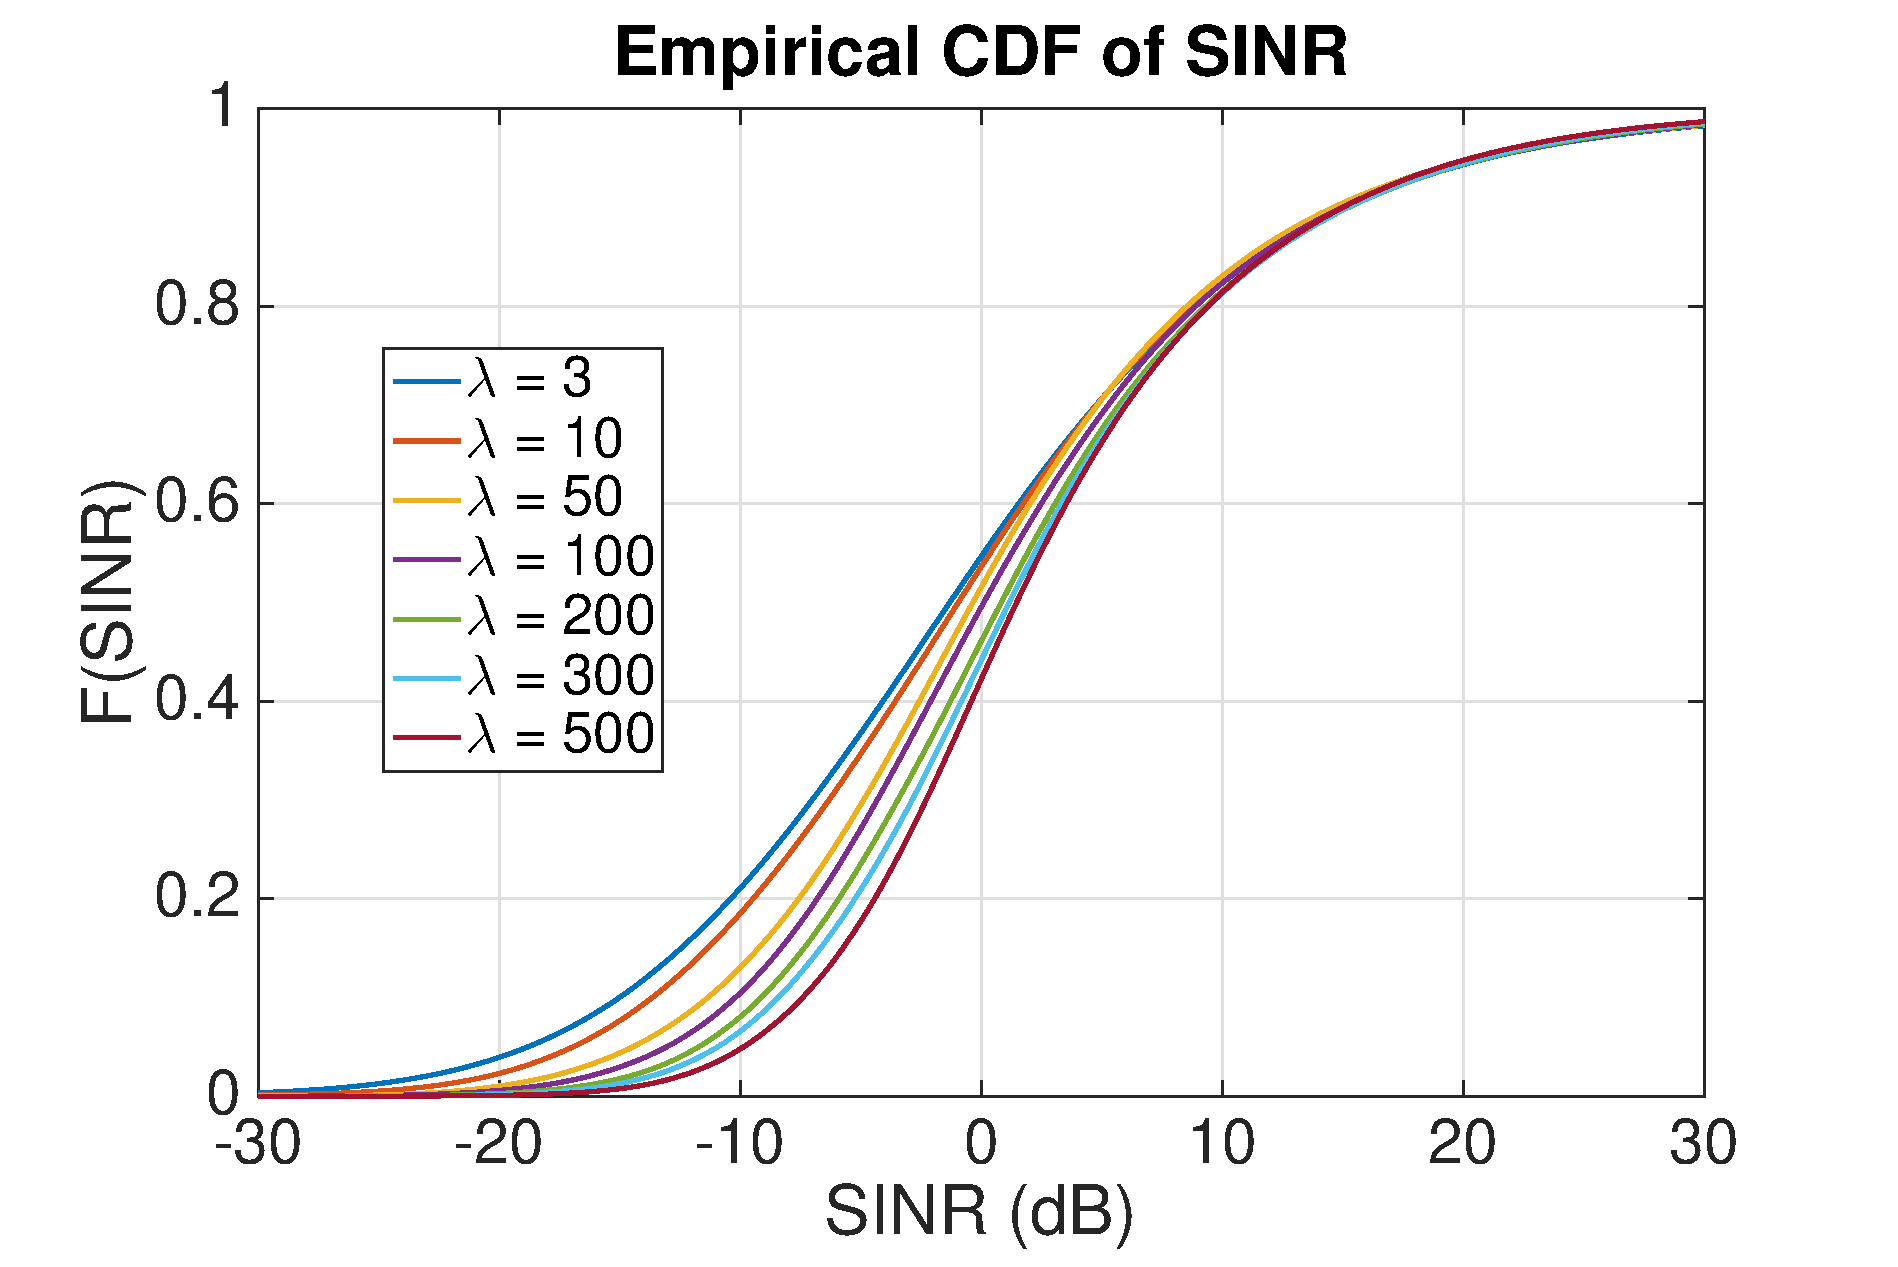
\includegraphics[width=10cm]{NBMax1000OutageProbCDFDeCorr200.eps}
\caption{CDF of SINR of MU when connecting to the nearest BS. De-Correlation Distance: 200m}
\label{Mode3}
\end{figure}


\begin{figure}
\centering
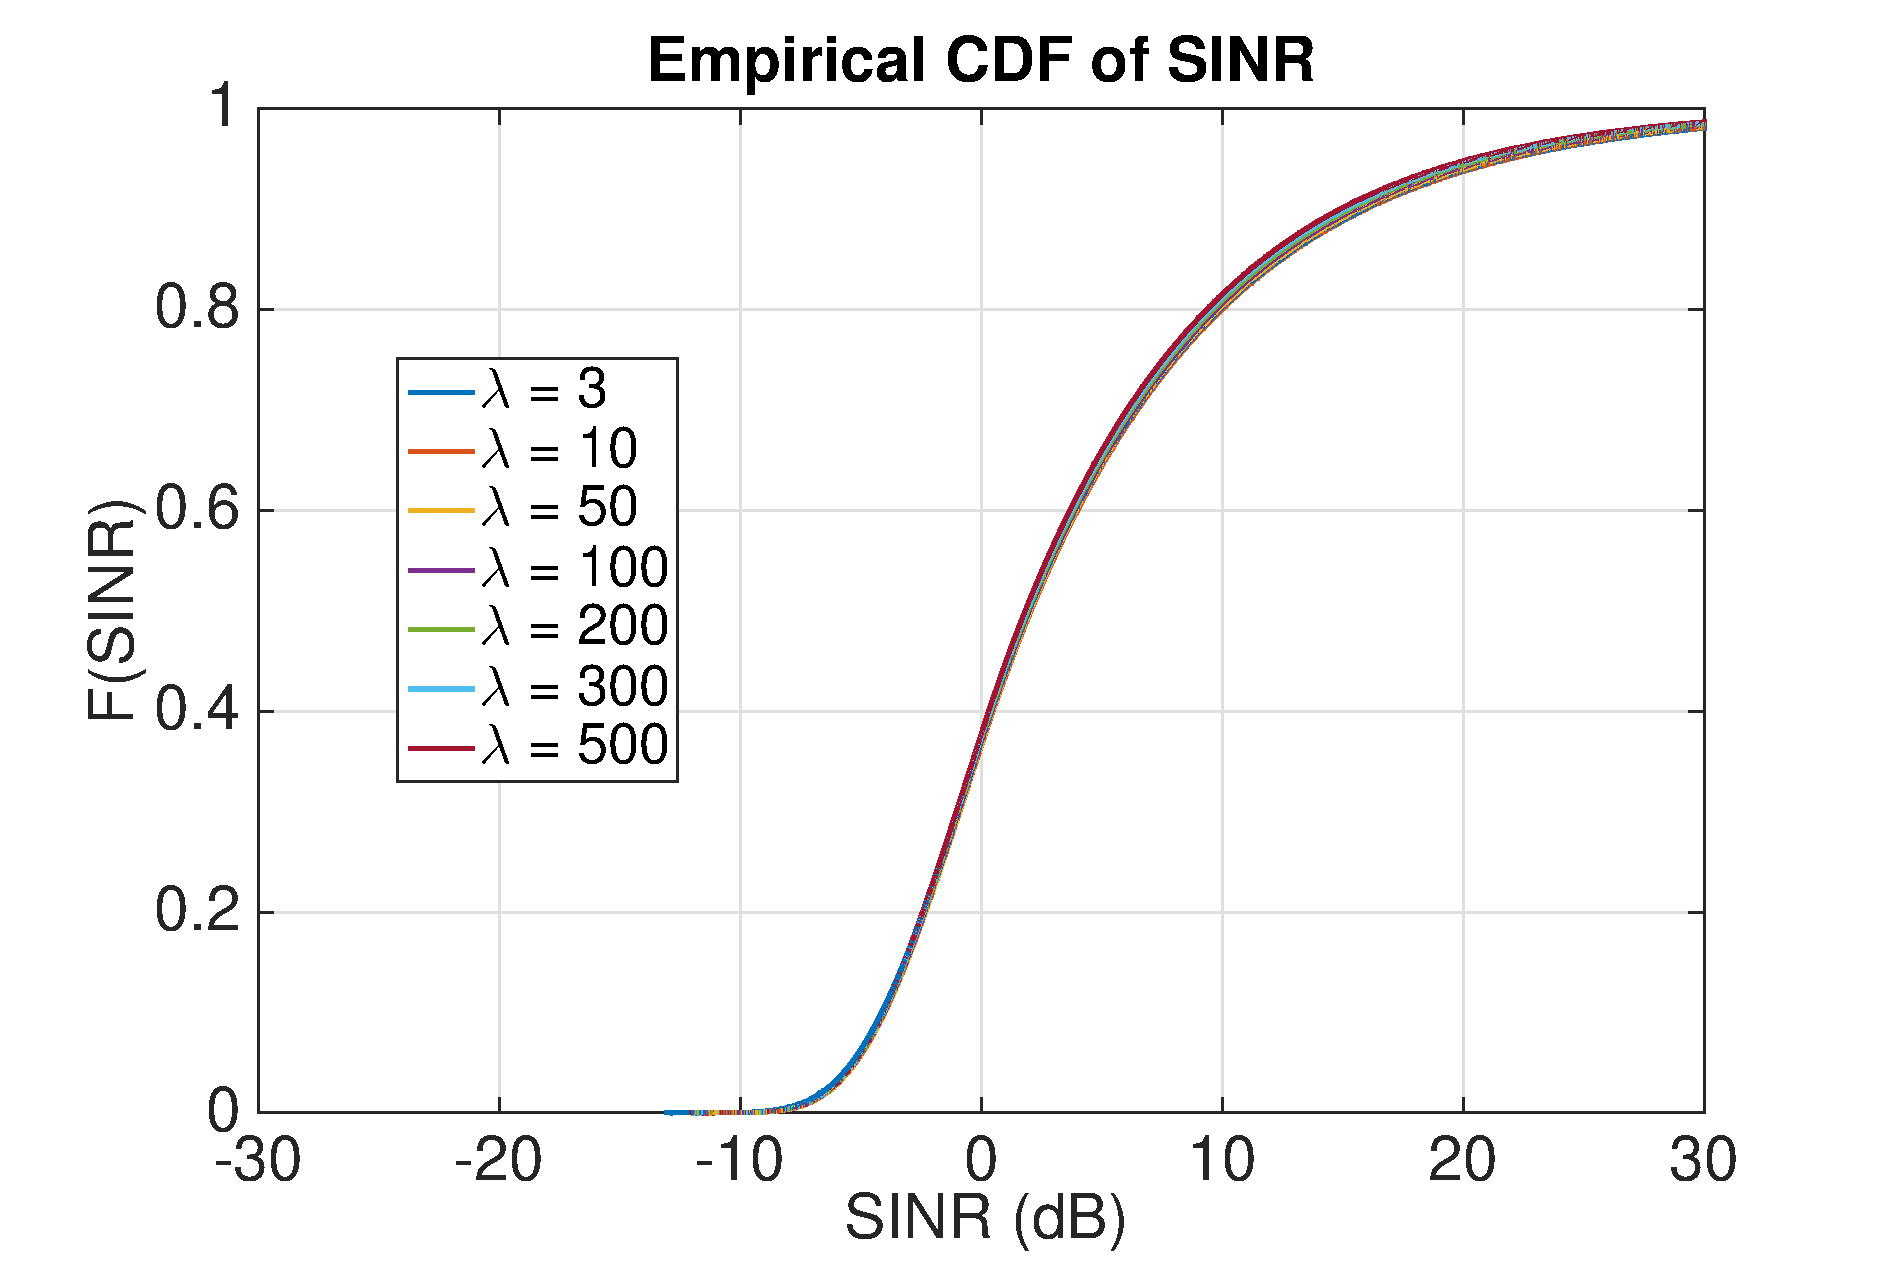
\includegraphics[width=10cm]{MaxMax1000OutageProbCDFiid.eps}
\caption{CDF of SINR of MU when connecting to the strongest BS. i.i.d. Shadow Fading}
\label{Mode12}
\end{figure}
\begin{figure}
\centering
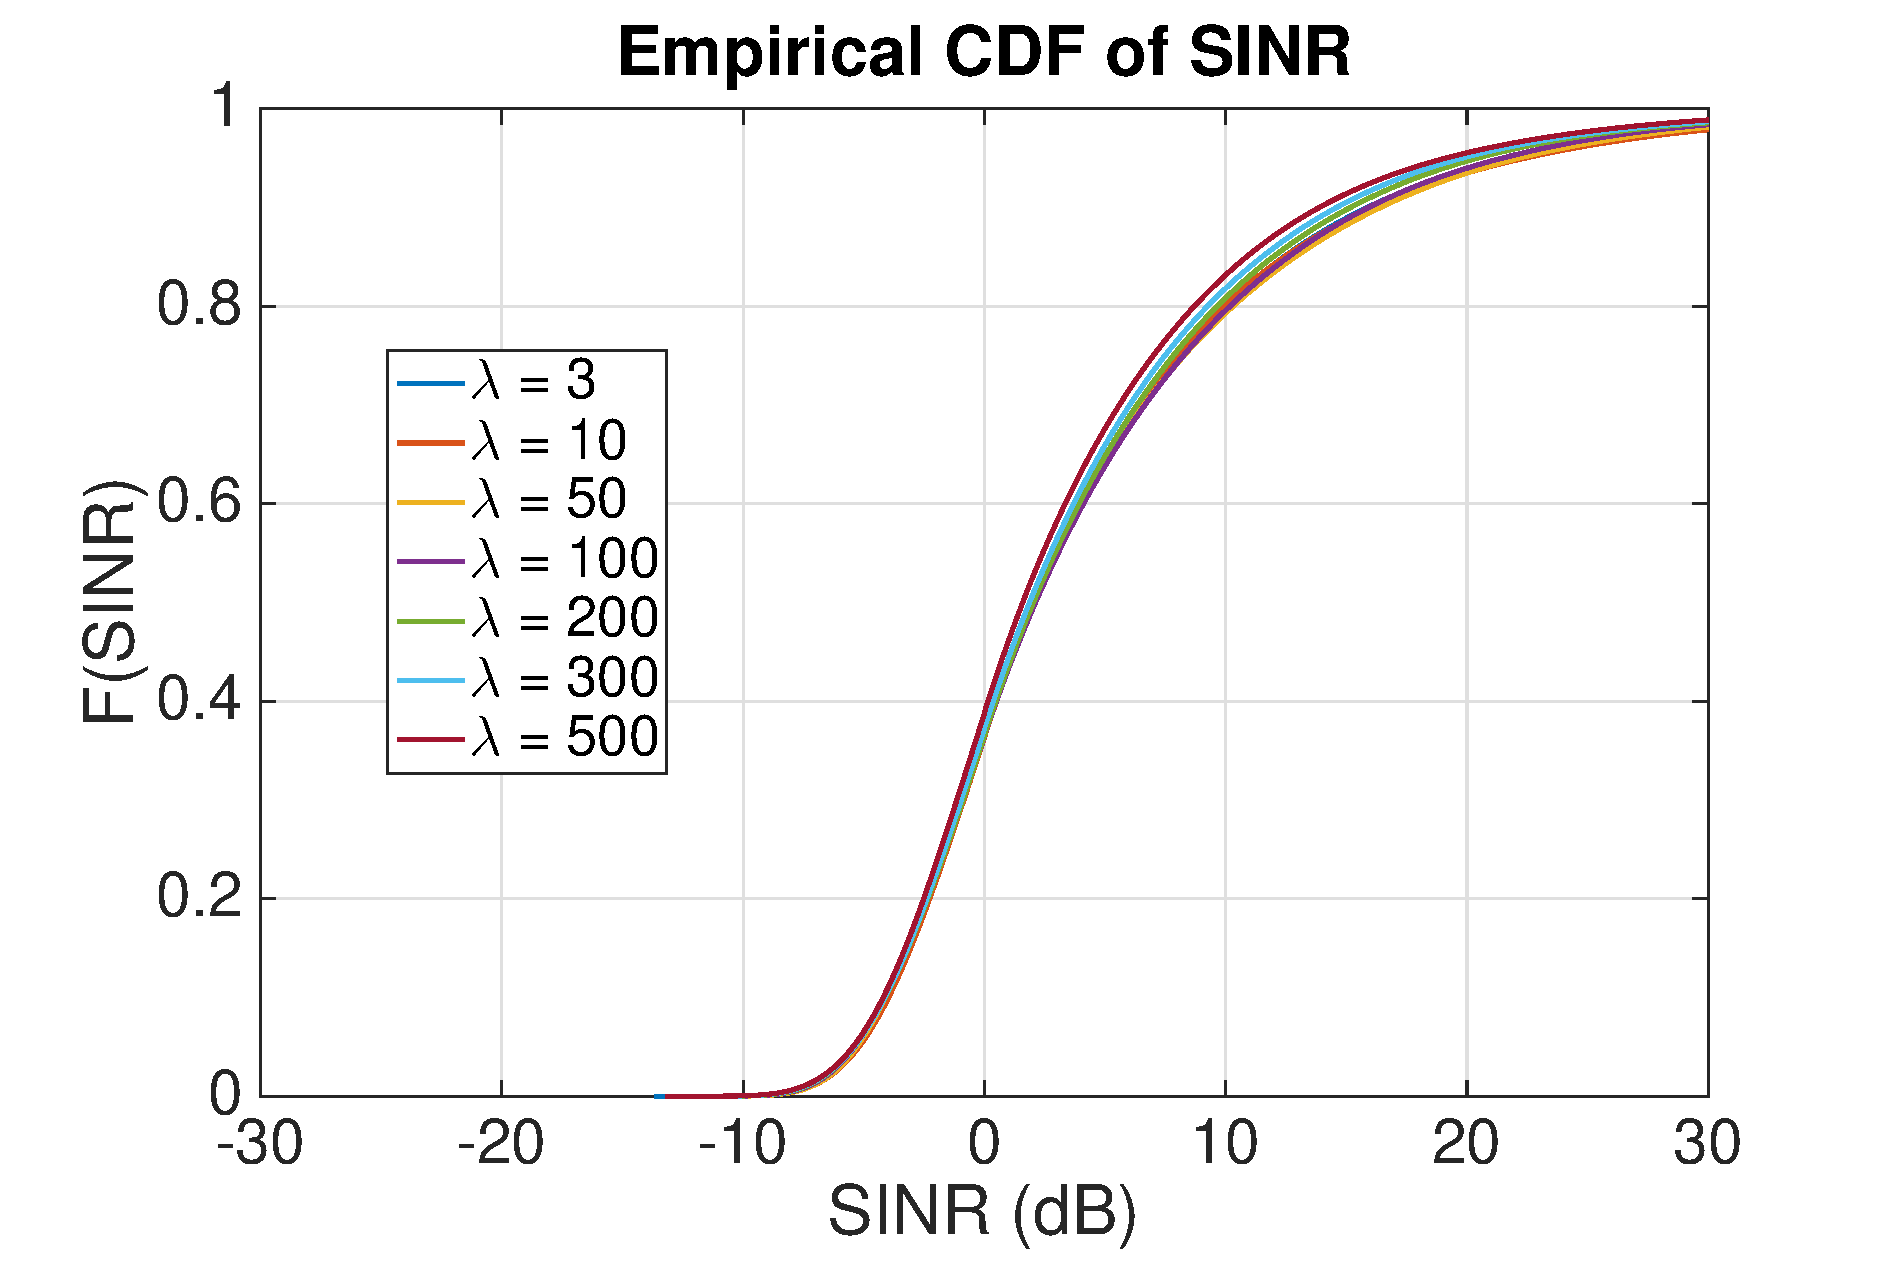
\includegraphics[width=10cm]{MaxMax1000OutageProbCDFDeCorr20.eps}
\caption{CDF of SINR of MU when connecting to the strongest BS. De-Correlation Distance: 20m}
\label{Mode22}
\end{figure}
\begin{figure}
\centering
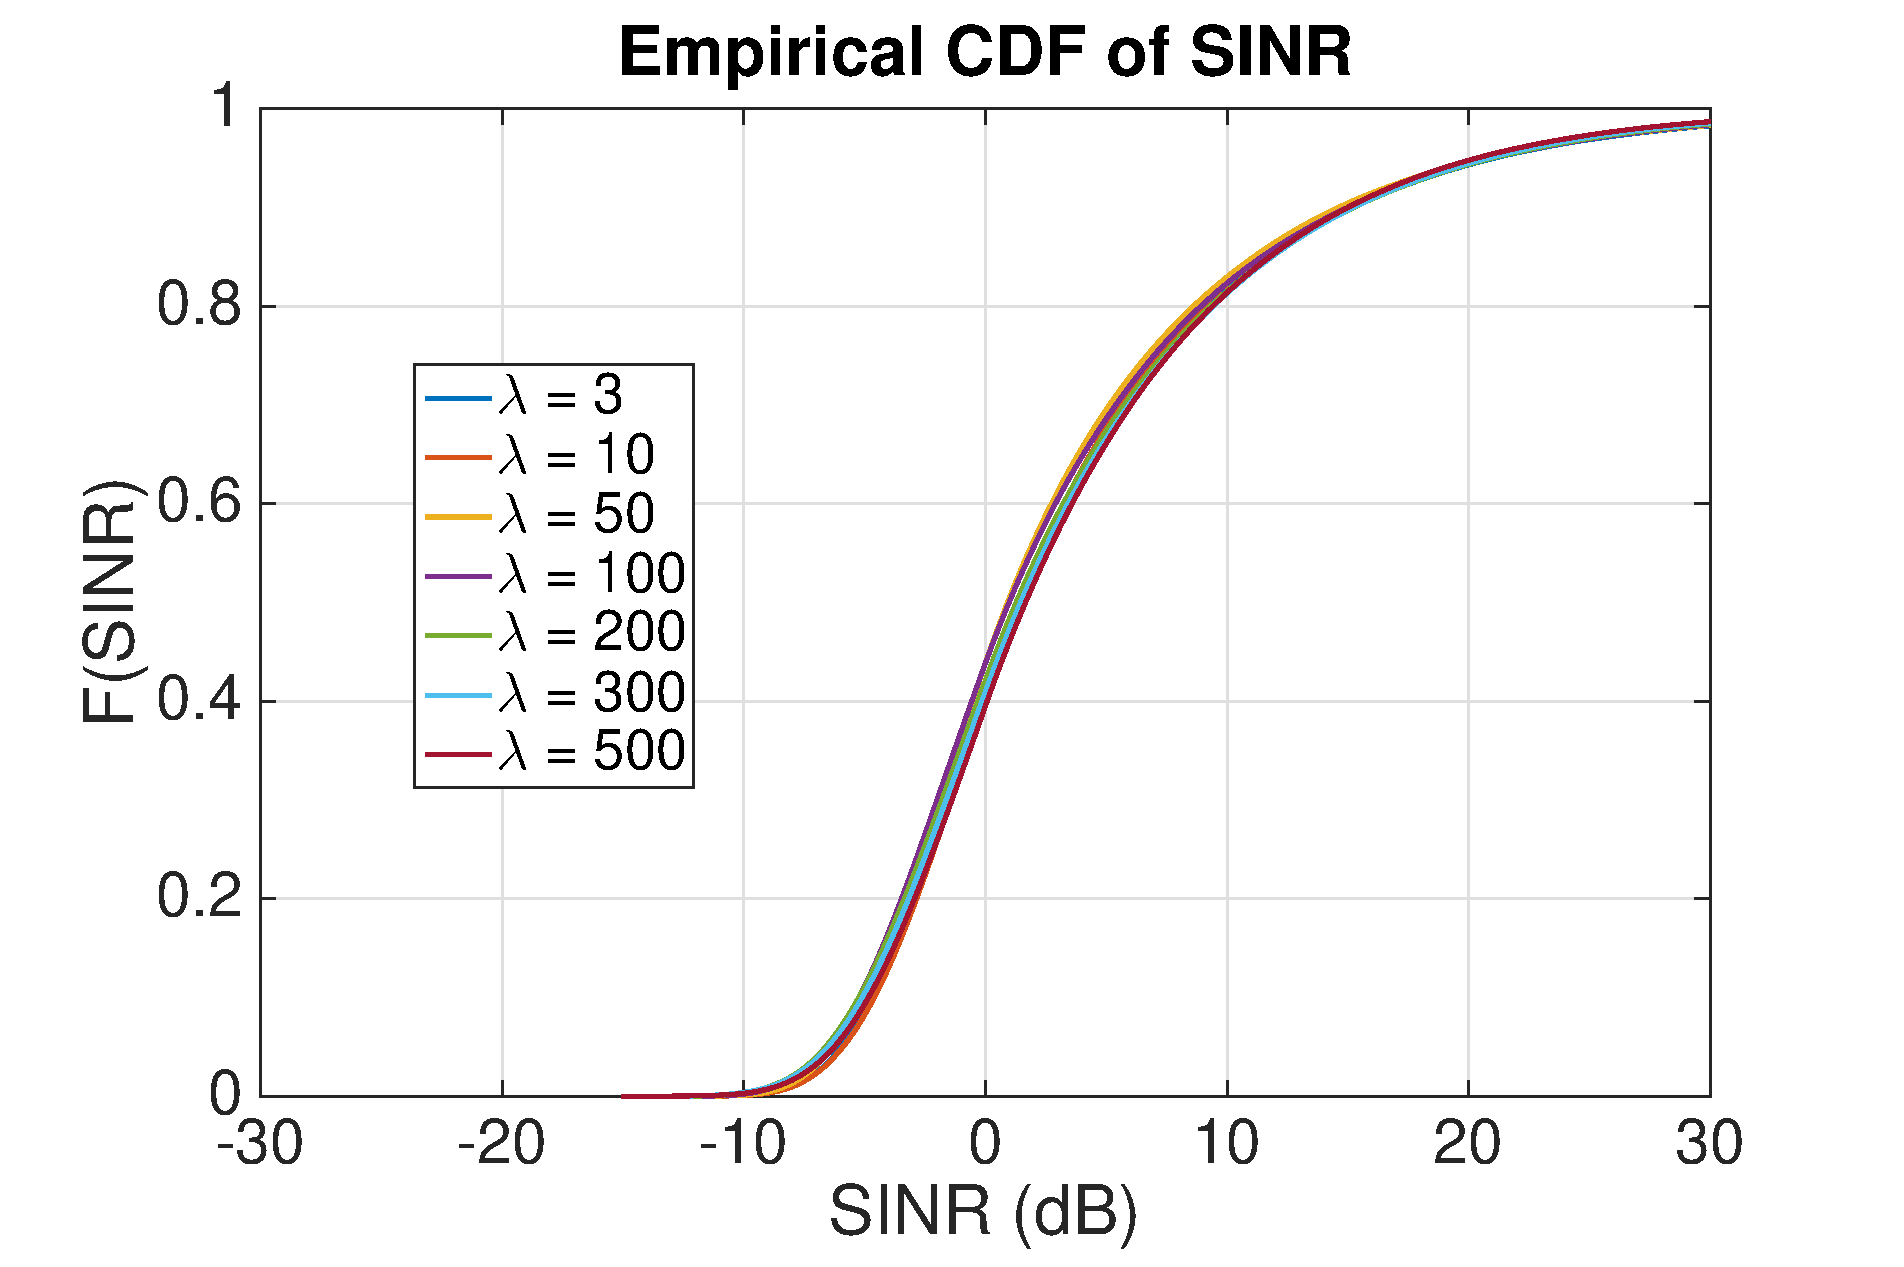
\includegraphics[width=10cm]{MaxMax1000OutageProbCDFDeCorr200.eps}
\caption{CDF of SINR of MU when connecting to the strongest BS. De-Correlation Distance: 200m}
\label{Mode32}
\end{figure}

\par For Random model, SINR distribution and outage probability of different BS densities are investigated for both nearest BS connection and strongest BS connection. Simulations are run for \emph{i.i.d.} shadow fading and correlated shadow fading. CDF of SINR are calculated and outage probability given SINR threshold $-5dB$ are presented for increasing BS densities. Figure. \ref{Mode1} \ref{Mode2} and \ref{Mode3} shows the SINR of MU when connecting to the nearest BS. From Figure. \ref{Mode1} and \ref{Mode2} we can see that the CDF are overlapping each other which means increasing BS density does not change the CDF of SINR. From this we can conclude that when the shadow fading is \emph{i.i.d.} or the De-Correlation distance of the correlated shadow fading is small, increasing BS will not improve the system performance in terms of outage probability. Figure. \ref{Mode3}  shows that when increasing BS density, CDF of SINR improves (curve moves toward the bottom-right corner). This suggests that when De-Correlation distance is large, increasing BS density will result in better system performance in terms of outage probability. Figure. \ref{fig: outprob1} shows the outage probability of different correlated shadow fading models and different BS densities when SINR threshold is set to $-5dB$. Blue and green bars suggest that increasing BS density will not decrease outage probability when shadow fading is \emph{i.i.d} or shadow fading has $20m$ De-Correlation distance. Yellow bars suggest that when the De-correlation distance is $200m$, increasing BS density will decrease outage probability. For example, when BS density is $3$, the outage probability is around $38\%$. Increasing BS density to $500$, the outage probability is decreased to $18\%$. From all above simulation results, we conclude that when De-Correlation distance is relatively large and MU is connecting to the nearest BS, increasing BS density will improve system performance in terms of decreasing outage probability.



\begin{figure}
\centering
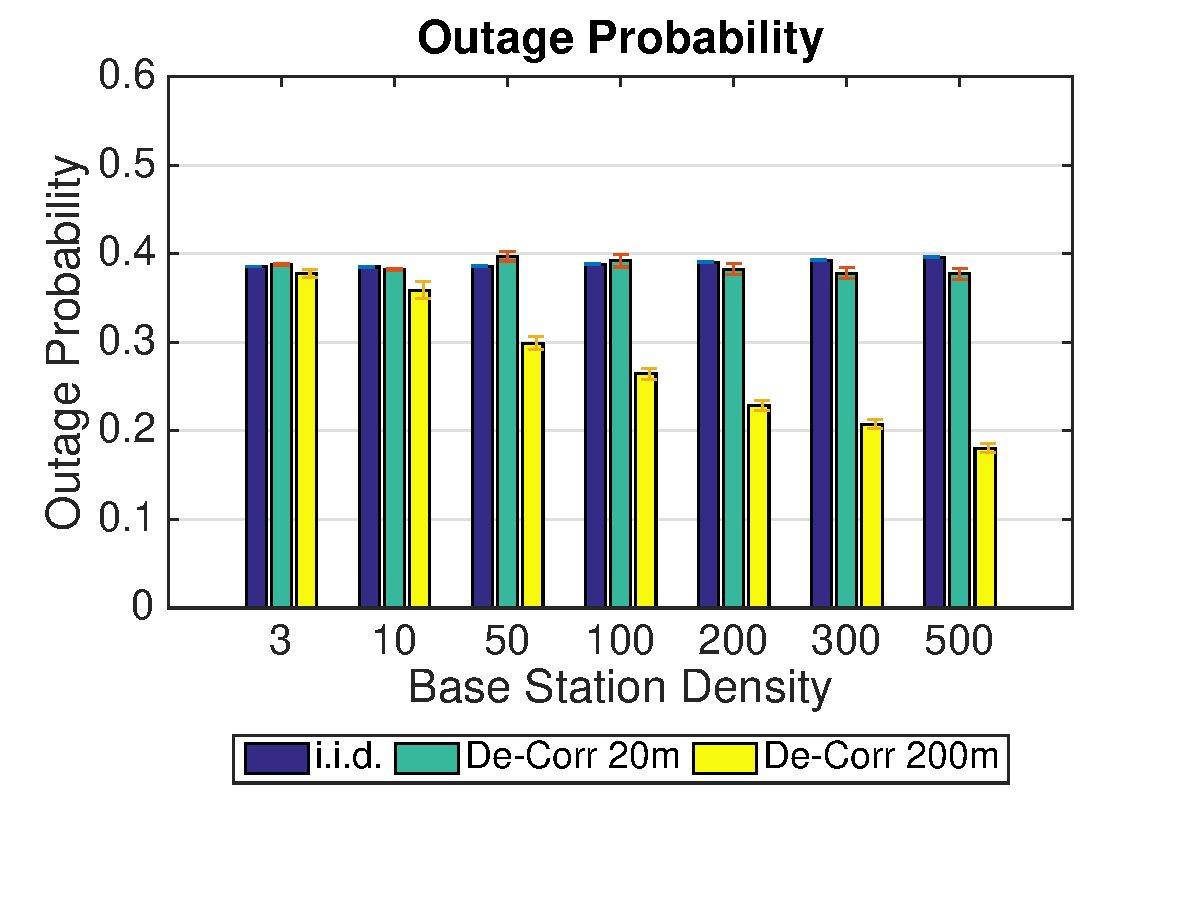
\includegraphics[width=10cm]{NBMax1000OutageProbThresh-5iid.eps}
\caption{Outage probability given SINR threshold to be $-5dB$}
\label{fig: outprob1}
\end{figure}
\begin{figure}
\centering
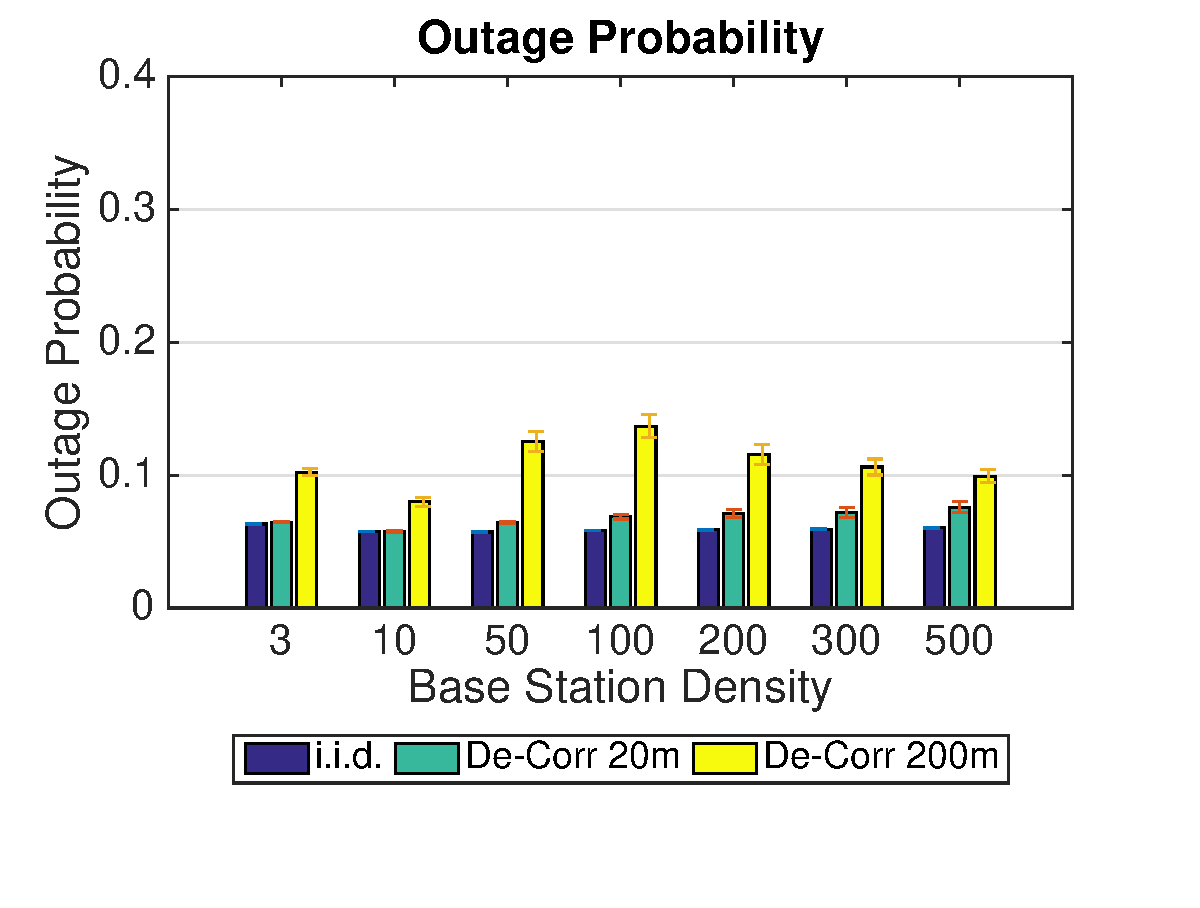
\includegraphics[width=10cm]{MaxMax1000OutageProbThresh-5iid.eps}
\caption{Outage probability given SINR threshold to be $-5dB$}
\label{fig: outprobs2}
\end{figure}
\begin{figure}
\centering
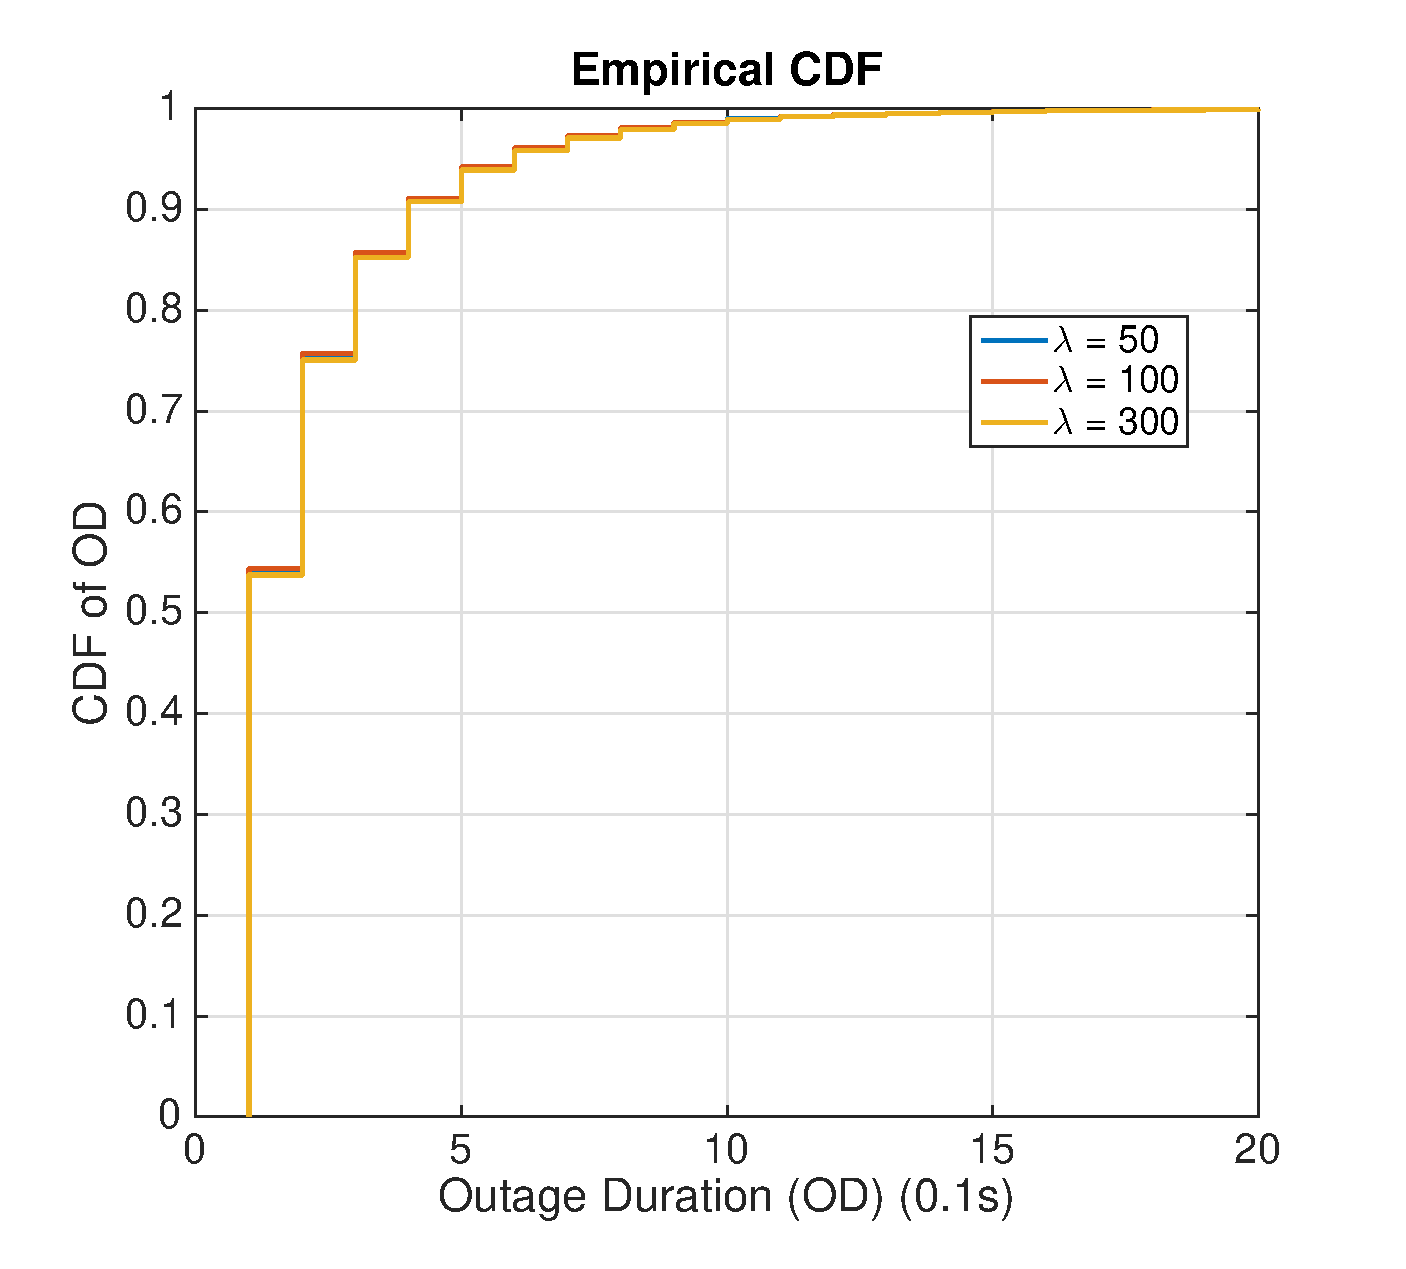
\includegraphics[width=10cm]{ODthresh-5iidNB.eps}
\caption{CDF of Outage Duration of MU when connecting to the Nearest BS with i.i.d. shadowing}
\label{iid1}
\end{figure}
\begin{figure}
\centering
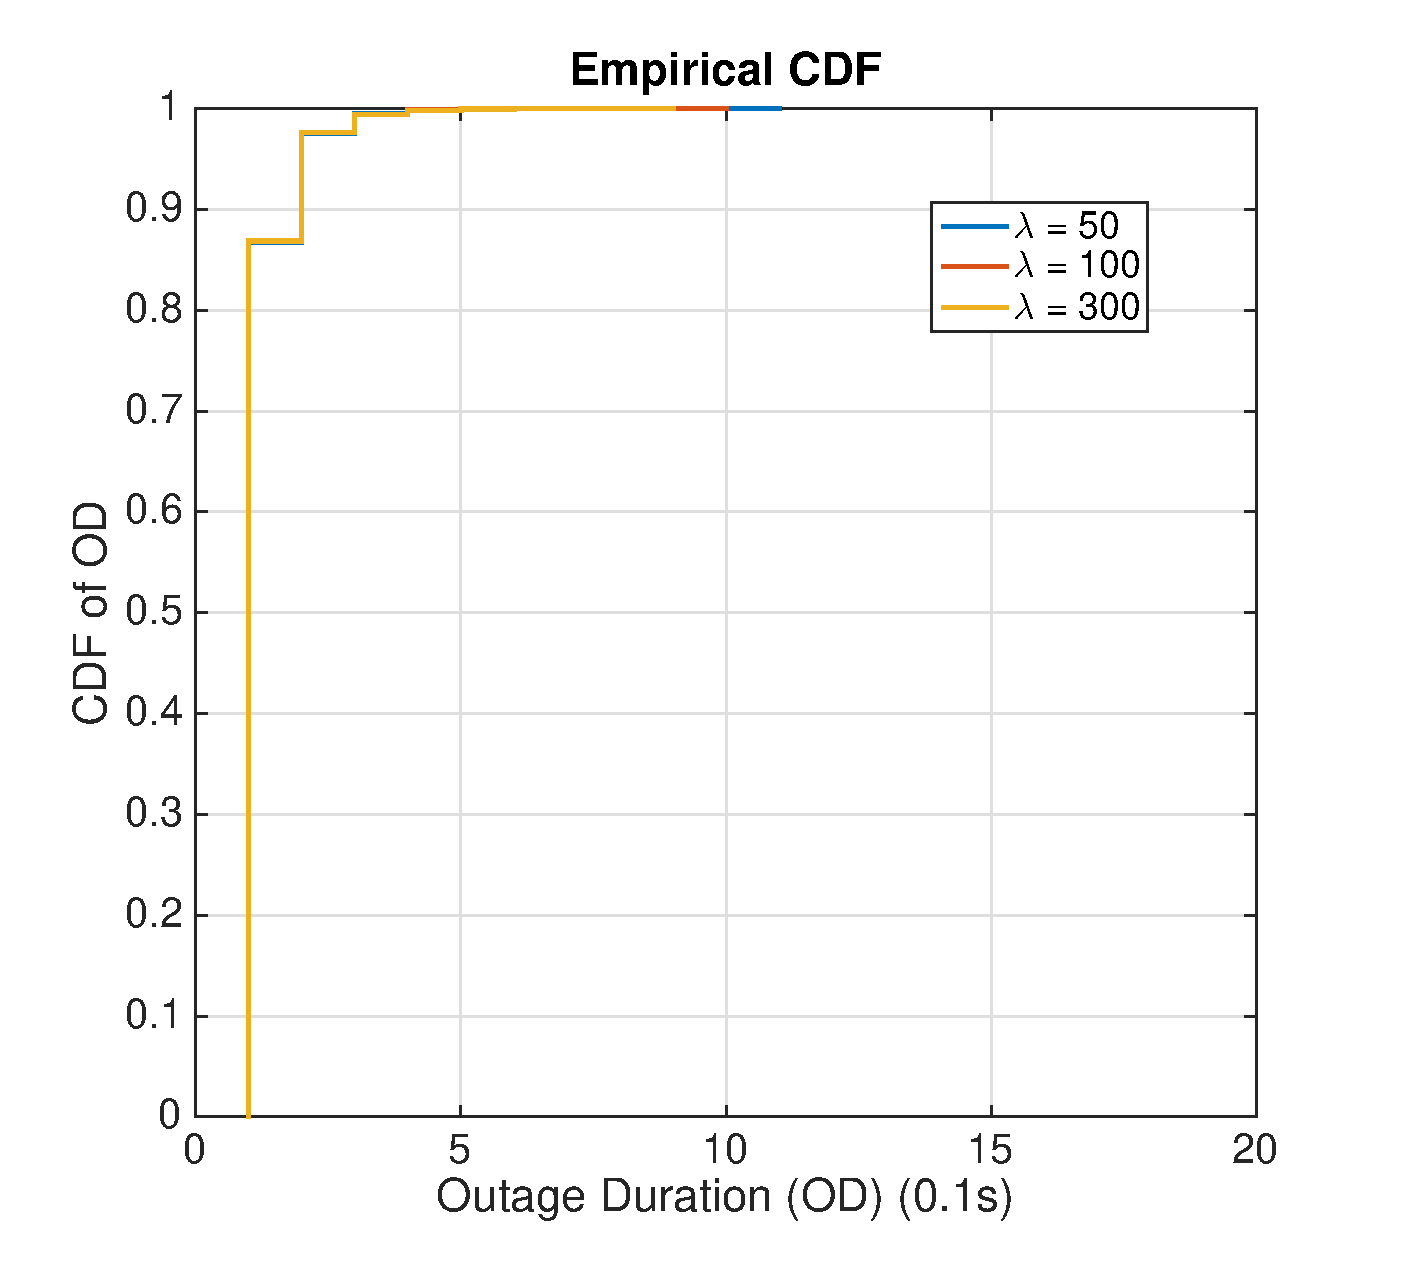
\includegraphics[width=10cm]{ODthresh-5iidMax.eps}
\caption{CDF of Outage Duration of MU when connecting to the Strongest BS with i.i.d. shadowing}
\label{iid2}
\end{figure}
\begin{figure}
\centering
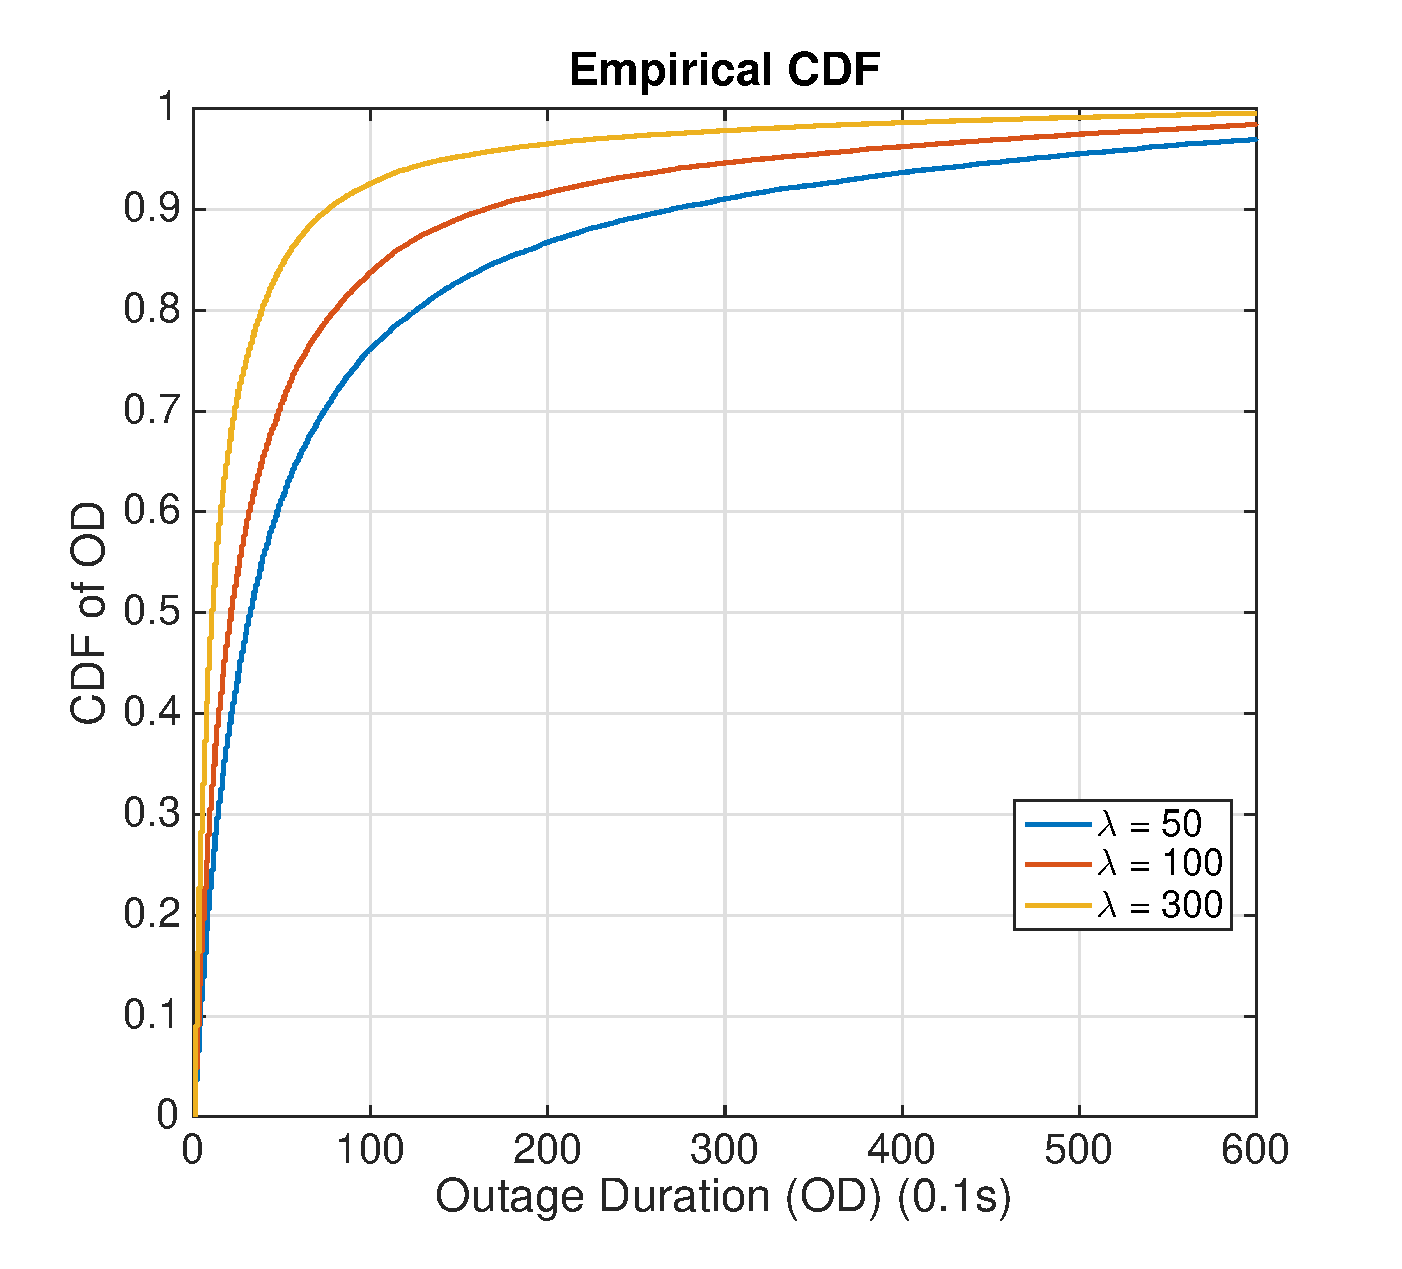
\includegraphics[width=10cm]{ODthresh-5DeCorr200NB.eps}
\caption{CDF of Outage Duration of MU when connecting to the Nearest BS with correlated shadowing (De-Correlation distance: 200m)}
\label{corr1}
\end{figure}
\begin{figure}
\centering
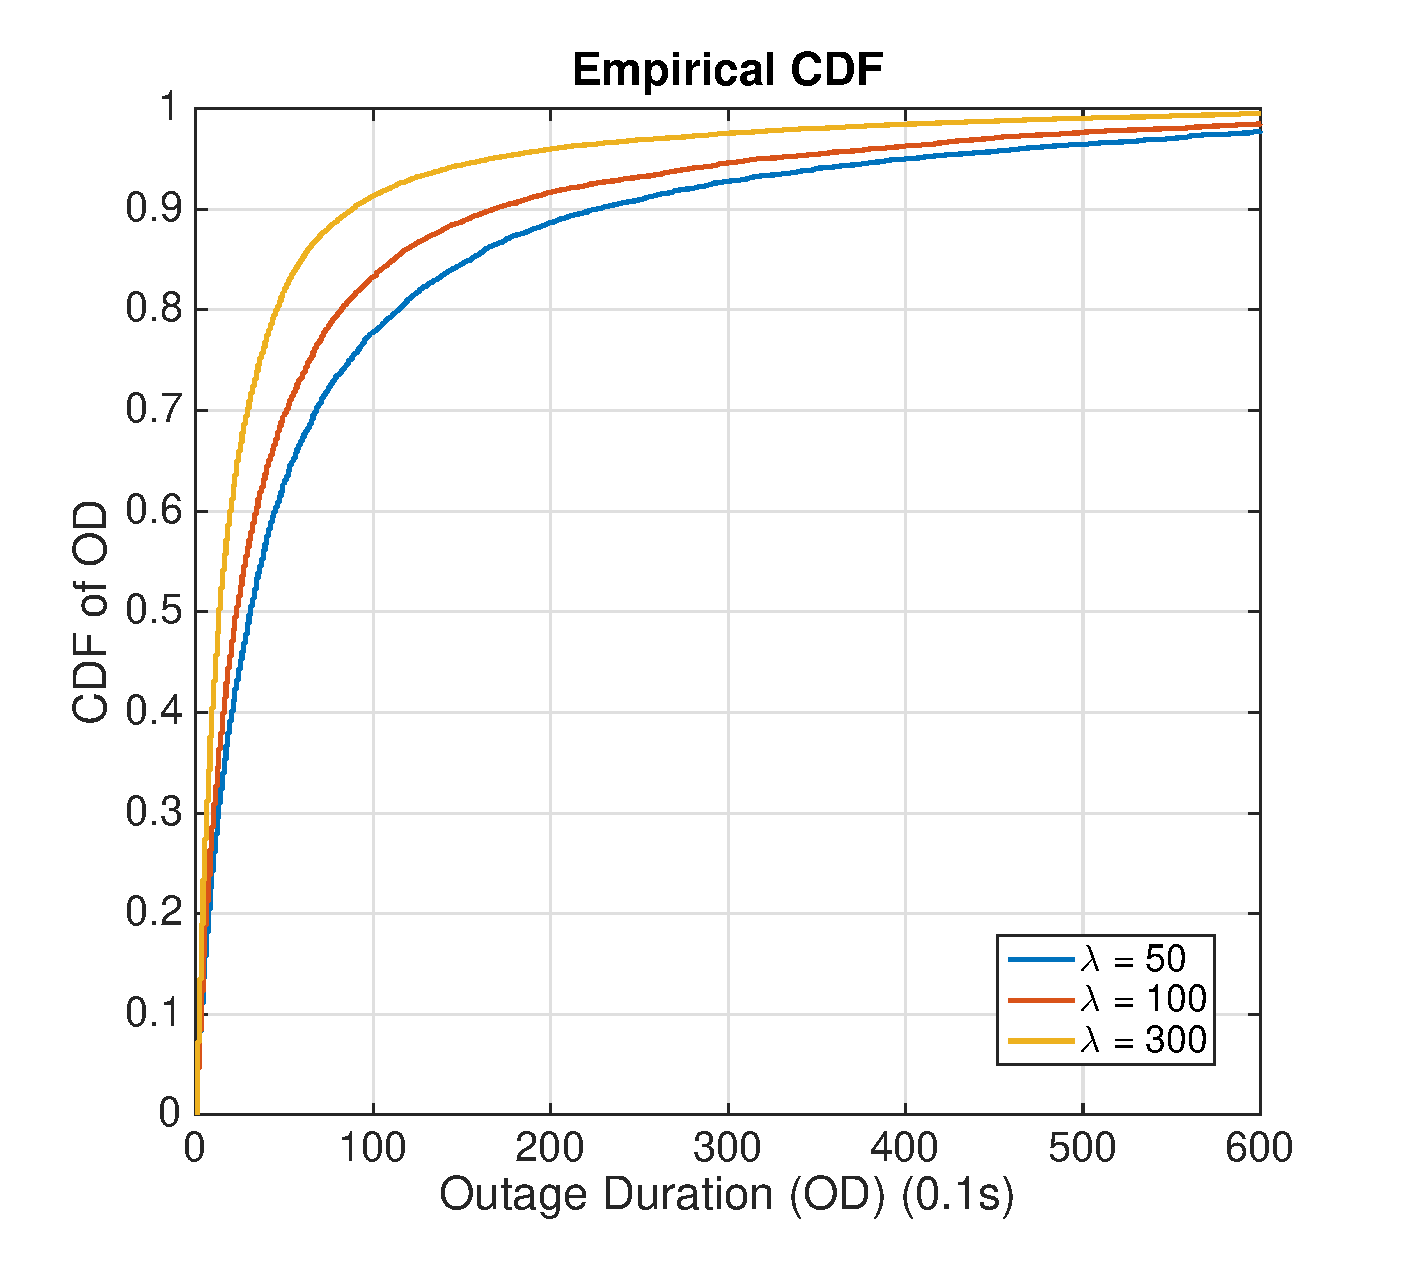
\includegraphics[width=10cm]{ODthresh-5DeCorr200Max.eps}
\caption{CDF of Outage Duration of MU when connecting to the Strongest BS with correlated shadowing (De-Correlation distance: 200m)}
\label{corr2}
\end{figure}
\par Next we move forward to investigate the system performance when the MU choose to connect to the BS which provides the strongest signal. Same simulations as the nearest BS scenario are run to study this scenario. Figure. \ref{Mode12} \ref{Mode22} and \ref{Mode32} shows the SINR of MU when connecting to the strongest BS. From subfigure \ref{Mode12}, \ref{Mode22} and \ref{Mode32} we can see that CDF of SINR almost overlap each other when increasing BS densities. This indicates that increasing BS density will not change CDF of SINR significantly. Figure. \ref{fig: outprobs2} shows outage probability result which is consistent with our aforementioned conclusion. For each shadow fading model, the difference of highest outage probability and lowest outage probability is less than $0.5$. Compare three different shadow fading models, we can conclude that when the MU is connecting to the strongest BS, long De-Correlation distance will harm the system performance in terms of outage probability (yellow bars are higher than green or blue bars). 
\par Comparing Figure. \ref{fig: outprob1} and Figure. \ref{fig: outprobs2}, we can see that with same BS density, when MU connecting to the strongest channel, the outage probabilities are lower for every shadow fading model. For example, with \emph{i.i.d.} shadow fading and BS density to be $50$, the outage probability of connecting to nearest BS is $38\%$ while that of connecting to strongest BS is $6\%$. For correlated shadow fading with De-Correlation distance being $200m$, take the BS density $50$ as an example, we found that the outage probability of connecting to nearest BS is around $30\%$, which is higher than that of connecting to strongest BS, which is $14\%$. This suggests given the same network setup, connecting to the BS which provides strongest channel will improve the system performance. 








\par Next, we will investigate the system performance form perspect of outage duration. We use Random Waypoint mobility model to model the user mobility. The parameters of the Random WayPoint model is given as in Table. \ref{RWP}. The MU speed is assume to be between $1m/s$ (pedestrian speed) to $20m/s$ (high way car speed). The MU pause interval is assumed to be uniformly between $0s$ to $60s$. The simulation time is set to be $0.1s$, which means for every $0.1s$ we check the MU's SINR to determine if it is still in the outage area or not.  The simulation result is showed in Figure. \ref{iid1}, \ref{corr1}, \ref{iid2} and \ref{corr2}. Comparing Figure. \ref{iid1} and Figure. \ref{corr1}, Figure. \ref{iid2} and Figure. \ref{corr2}, we can see that when the channel is experiencing i.i.d. shadow fading, the outage duration is usually less than $2s$. However,  when the channel is under correlated shadow fading with De-Correlation distance equal to $200m$, the outage duration can be longer than $30s$. Therefore, we can conclude that correlated shadow fading brings long outage duration to the system. Comparing Figure. \ref{iid1} and Figure. \ref{iid2}, we found that with i.i.d. shadow fading, connecting to strongest BS will reduce the outage duration.  Nevertheless, Figure. \ref{corr1} and Figure. \ref{corr2} suggests that changing connection strategy will not improve the outage duration in terms of distribution, although connecting to strongest BS will reduce outage probability. Both Figure. \ref{corr1} and Figure. \ref{corr2} indicate that increasing BS density will reduce long outage duration. For example, in Figure. \ref{corr1}, when the BS density increase from $50$ to $300$, the probability of outage duration longer than $10s$ is reduced from $24\%$ to $7\%$. In contrast, for i.i.d. shadow fading, increase BS density will not change the distribution of outage duration, which is confirmed by Figure. \ref{iid1} and Figure. \ref{iid2}. All CDF curve of outage duration overlap each other when BS density changes. 
\begin{table}
\centering
\caption{\label{RWP}Random Waypoint Mobility Model Parameters}

\begin{tabular}{|c|c|}

\hline
Speed Interval & $1 - 20m/s$\\
\hline
Pause Interval & $0 - 60s$\\
\hline
Simulation Time & $0.1s$\\
\hline
\end{tabular}

\end{table}

\section{Conclusions}
\label{ch4:Conclusion}
Shadow fading is large-scale fading which can cause significant received power loss for a wide area. In general, shadow fading is considered to be i.i.d. to simplify the analysis. However, this is not the real case. In reality, shadow fading at two different positions are correlated to each other. Correlated shadow fading will result in correlated long outage durations. Power outage will lead to connection loss and/or packet loss which is harmful to MUs, especially to those who are using real-time applications such as video conferencing. To investigate a multi-cell system performance given correlated shadow fading, simulations are run to study the outage probability and outage duration distribution. First of all, the probability of two different BS layout: Grid Layout and Random Layout are investigated. We found that Grid Layout performs better than Random Layout. Secondly, outage probability given different BS densities and two different connecting strategies: nearest BS and strongest BS, are simulated. We conclude that connecting to strongest BS will reduce the outage probability comparing with nearest BS. Increasing BS density will not reduce outage probability when MU is connecting to the strongest BS. However, when MU is connecting to the nearest BS and the De-Correlation distance of correlated shadow fading is large enough, increasing BS density will reduce the outage probability, therefore improve the system performance. At last, we investigate system performance in terms of outage duration. The simulation results show that correlated shadow fading will result in long outage duration. Increasing BS density will efficiently reduce the percentage of long outage duration.
 

